% Options for packages loaded elsewhere
% Options for packages loaded elsewhere
\PassOptionsToPackage{unicode}{hyperref}
\PassOptionsToPackage{hyphens}{url}
\PassOptionsToPackage{dvipsnames,svgnames,x11names}{xcolor}
%
\documentclass[
  11pt,
  us-letterpaper,
  DIV=11,
  numbers=noendperiod]{scrartcl}
\usepackage{xcolor}
\usepackage[margin=1in]{geometry}
\usepackage{amsmath,amssymb}
\setcounter{secnumdepth}{5}
\usepackage{iftex}
\ifPDFTeX
  \usepackage[T1]{fontenc}
  \usepackage[utf8]{inputenc}
  \usepackage{textcomp} % provide euro and other symbols
\else % if luatex or xetex
  \usepackage{unicode-math} % this also loads fontspec
  \defaultfontfeatures{Scale=MatchLowercase}
  \defaultfontfeatures[\rmfamily]{Ligatures=TeX,Scale=1}
\fi
\usepackage{lmodern}
\ifPDFTeX\else
  % xetex/luatex font selection
  \setmainfont[]{Times New Roman}
  \setsansfont[]{Arial}
  \setmonofont[Scale=0.78]{Liberation Mono}
\fi
% Use upquote if available, for straight quotes in verbatim environments
\IfFileExists{upquote.sty}{\usepackage{upquote}}{}
\IfFileExists{microtype.sty}{% use microtype if available
  \usepackage[]{microtype}
  \UseMicrotypeSet[protrusion]{basicmath} % disable protrusion for tt fonts
}{}
\usepackage{setspace}
\makeatletter
\@ifundefined{KOMAClassName}{% if non-KOMA class
  \IfFileExists{parskip.sty}{%
    \usepackage{parskip}
  }{% else
    \setlength{\parindent}{0pt}
    \setlength{\parskip}{6pt plus 2pt minus 1pt}}
}{% if KOMA class
  \KOMAoptions{parskip=half}}
\makeatother
% Make \paragraph and \subparagraph free-standing
\makeatletter
\ifx\paragraph\undefined\else
  \let\oldparagraph\paragraph
  \renewcommand{\paragraph}{
    \@ifstar
      \xxxParagraphStar
      \xxxParagraphNoStar
  }
  \newcommand{\xxxParagraphStar}[1]{\oldparagraph*{#1}\mbox{}}
  \newcommand{\xxxParagraphNoStar}[1]{\oldparagraph{#1}\mbox{}}
\fi
\ifx\subparagraph\undefined\else
  \let\oldsubparagraph\subparagraph
  \renewcommand{\subparagraph}{
    \@ifstar
      \xxxSubParagraphStar
      \xxxSubParagraphNoStar
  }
  \newcommand{\xxxSubParagraphStar}[1]{\oldsubparagraph*{#1}\mbox{}}
  \newcommand{\xxxSubParagraphNoStar}[1]{\oldsubparagraph{#1}\mbox{}}
\fi
\makeatother


\usepackage{longtable,booktabs,array}
\newcounter{none} % for unnumbered tables
\usepackage{calc} % for calculating minipage widths
% Correct order of tables after \paragraph or \subparagraph
\usepackage{etoolbox}
\makeatletter
\patchcmd\longtable{\par}{\if@noskipsec\mbox{}\fi\par}{}{}
\makeatother
% Allow footnotes in longtable head/foot
\IfFileExists{footnotehyper.sty}{\usepackage{footnotehyper}}{\usepackage{footnote}}
\makesavenoteenv{longtable}
\usepackage{graphicx}
\makeatletter
\newsavebox\pandoc@box
\newcommand*\pandocbounded[1]{% scales image to fit in text height/width
  \sbox\pandoc@box{#1}%
  \Gscale@div\@tempa{\textheight}{\dimexpr\ht\pandoc@box+\dp\pandoc@box\relax}%
  \Gscale@div\@tempb{\linewidth}{\wd\pandoc@box}%
  \ifdim\@tempb\p@<\@tempa\p@\let\@tempa\@tempb\fi% select the smaller of both
  \ifdim\@tempa\p@<\p@\scalebox{\@tempa}{\usebox\pandoc@box}%
  \else\usebox{\pandoc@box}%
  \fi%
}
% Set default figure placement to htbp
\def\fps@figure{htbp}
\makeatother


% definitions for citeproc citations
\NewDocumentCommand\citeproctext{}{}
\NewDocumentCommand\citeproc{mm}{%
  \begingroup\def\citeproctext{#2}\cite{#1}\endgroup}
\makeatletter
 % allow citations to break across lines
 \let\@cite@ofmt\@firstofone
 % avoid brackets around text for \cite:
 \def\@biblabel#1{}
 \def\@cite#1#2{{#1\if@tempswa , #2\fi}}
\makeatother
\newlength{\cslhangindent}
\setlength{\cslhangindent}{1.5em}
\newlength{\csllabelwidth}
\setlength{\csllabelwidth}{3em}
\newenvironment{CSLReferences}[2] % #1 hanging-indent, #2 entry-spacing
 {\begin{list}{}{%
  \setlength{\itemindent}{0pt}
  \setlength{\leftmargin}{0pt}
  \setlength{\parsep}{0pt}
  % turn on hanging indent if param 1 is 1
  \ifodd #1
   \setlength{\leftmargin}{\cslhangindent}
   \setlength{\itemindent}{-1\cslhangindent}
  \fi
  % set entry spacing
  \setlength{\itemsep}{#2\baselineskip}}}
 {\end{list}}
\usepackage{calc}
\newcommand{\CSLBlock}[1]{\hfill\break\parbox[t]{\linewidth}{\strut\ignorespaces#1\strut}}
\newcommand{\CSLLeftMargin}[1]{\parbox[t]{\csllabelwidth}{\strut#1\strut}}
\newcommand{\CSLRightInline}[1]{\parbox[t]{\linewidth - \csllabelwidth}{\strut#1\strut}}
\newcommand{\CSLIndent}[1]{\hspace{\cslhangindent}#1}



\setlength{\emergencystretch}{3em} % prevent overfull lines

\providecommand{\tightlist}{%
  \setlength{\itemsep}{0pt}\setlength{\parskip}{0pt}}



 


\KOMAoption{captions}{tableheading}
\setkomafont{disposition}{\normalfont\bfseries}
\setkomafont{descriptionlabel}{\normalfont\bfseries}
\setkomafont{caption}{\small}
\setkomafont{captionlabel}{\normalfont\small\bfseries}
\usepackage{etoolbox}
\AtBeginEnvironment{longtable}{\small}
\usepackage[htt]{hyphenat}
\usepackage{seqsplit}
\usepackage{xurl}
\makeatletter
\@ifpackageloaded{caption}{}{\usepackage{caption}}
\AtBeginDocument{%
\ifdefined\contentsname
  \renewcommand*\contentsname{Table of contents}
\else
  \newcommand\contentsname{Table of contents}
\fi
\ifdefined\listfigurename
  \renewcommand*\listfigurename{List of Figures}
\else
  \newcommand\listfigurename{List of Figures}
\fi
\ifdefined\listtablename
  \renewcommand*\listtablename{List of Tables}
\else
  \newcommand\listtablename{List of Tables}
\fi
\ifdefined\figurename
  \renewcommand*\figurename{Figure}
\else
  \newcommand\figurename{Figure}
\fi
\ifdefined\tablename
  \renewcommand*\tablename{Table}
\else
  \newcommand\tablename{Table}
\fi
}
\@ifpackageloaded{float}{}{\usepackage{float}}
\floatstyle{ruled}
\@ifundefined{c@chapter}{\newfloat{codelisting}{h}{lop}}{\newfloat{codelisting}{h}{lop}[chapter]}
\floatname{codelisting}{Listing}
\newcommand*\listoflistings{\listof{codelisting}{List of Listings}}
\makeatother
\makeatletter
\makeatother
\makeatletter
\@ifpackageloaded{caption}{}{\usepackage{caption}}
\@ifpackageloaded{subcaption}{}{\usepackage{subcaption}}
\makeatother
\usepackage{bookmark}
\IfFileExists{xurl.sty}{\usepackage{xurl}}{} % add URL line breaks if available
\urlstyle{same}
% fallback for those not using the hyperref driver hyperxmp:
\makeatletter
\@ifundefined{xmpquote}{\newcommand{\xmpquote}[1]{#1}}{}
\makeatother
\hypersetup{
  pdftitle={Phenotype Conflation and Partner-Conditioned Evaluation in Zero-Shot Protein-Protein Interaction Benchmarks},
  pdfauthor={Emilio A. Venegas},
  pdfkeywords={\xmpquote{Protein Language
Models}, \xmpquote{Protein-Protein Interactions}, \xmpquote{Deep
Mutational Scanning}, \xmpquote{Assay Provenance}, \xmpquote{Quaternary
Interfaces}, \xmpquote{Benchmarking Defect}, \xmpquote{Partner
Specificity}},
  colorlinks=true,
  linkcolor={blue},
  filecolor={Maroon},
  citecolor={blue},
  urlcolor={blue},
  pdfcreator={LaTeX via pandoc}}


\title{Phenotype Conflation and Partner-Conditioned Evaluation in
Zero-Shot Protein-Protein Interaction Benchmarks}
\author{Emilio A. Venegas}
\date{}
\begin{document}
\maketitle
\begin{abstract}
Zero-shot single-chain protein language models (PLMs) such as ESM-1v,
ESM-2, and ESM-Cambrian (ESMC) are frequently benchmarked on deep
mutational scanning (DMS) binding assays, achieving reported rank
correlations \(\rho \approx 0.35\text{--}0.48\). These correlations are
often interpreted as evidence that single-sequence masked language
modeling captures intermolecular binding physics and quaternary contact
energetics. In this work, we demonstrate that benchmark performance can
be strongly confounded by target-intrinsic expression and folding
stability. In high-throughput selection assays, mutations that
destabilize monomer folding impair cell-surface presentation or cellular
abundance, indirectly eliminating partner binding and inflating
zero-shot scores through monomer-survival prediction. Through an
exhaustive provenance audit of deep mutational scanning benchmarks, we
show that widely pooled datasets conflate direct display-binding
measurements with expression-uncoupled assays, cross-study merges, and
cellular fitness proxies. In strictly matched display assays where
monomer surface expression and complex binding are measured on the
identical mutant library (SARS-CoV-2 RBD and HLA-A*02:01), sequence-only
PLM binding correlations at quaternary interfaces attenuate
substantially once monomer expression is controlled
(\(\rho_{\text{partial}} \approx 0.00\text{--}0.14\)). In contrast, 3D
structure-conditioned models (ProteinMPNN) retain robust interface
binding signal (\(\rho_{\text{partial}} = +0.202\)). Finally, we
demonstrate that evaluating single-chain PLMs on single-partner binding
readouts cannot distinguish target viability from partner-specific
binding, and we formalize a four-stage protocol for partner-conditioned
specificity benchmarks.
\end{abstract}


\setstretch{1.25}
\section{Introduction}\label{sec-intro}

Transformer-based protein language models (PLMs) trained on evolutionary
sequence databases via masked language modeling---such as ESM-2
(\citeproc{ref-lin2023evolutionary}{Lin et al. 2023}) and ESM-Cambrian
(ESMC) (\citeproc{ref-hayes2024simulating}{Hayes et al. 2025})---have
emerged as standard tools for zero-shot variant effect prediction and
protein engineering (\citeproc{ref-rives2021biological}{Rives et al.
2021}; \citeproc{ref-meier2021language}{Meier et al. 2021};
\citeproc{ref-hie2022evolutionary}{Hie et al. 2022}). In standard
evaluation protocols, single-chain masked log-odds ratios
\(\Delta \log p(x)\) are computed across deep mutational scanning (DMS)
datasets compiled in public benchmark suites such as ProteinGym
(\citeproc{ref-notin2023proteingym}{Notin et al. 2023}) and SKEMPI 2.0
(\citeproc{ref-jankauskaite2019skempi}{Jankauskaitė et al. 2019}).

On these benchmarks, zero-shot PLMs and evolutionary models
(\citeproc{ref-lin2023evolutionary}{Lin et al. 2023};
\citeproc{ref-rao2021msa}{Rao et al. 2021}) are reported to achieve
moderate-to-high rank correlations on protein-protein interaction (PPI)
and complex binding affinity assays (\(\rho \approx 0.35\text{--}0.48\))
(\citeproc{ref-notin2023proteingym}{Notin et al. 2023}). These
correlations have fostered the assumption that Transformer architectures
trained exclusively on single-chain sequences implicitly capture the
biophysics of intermolecular quaternary contacts and binding energetics
(\citeproc{ref-notin2023proteingym}{Notin et al. 2023};
\citeproc{ref-sledzieski2021dscript}{Sledzieski et al. 2021}).

In this work, we show that this assumption is vulnerable to a systematic
experimental confound: high-throughput binding selection platforms
(e.g., yeast surface display, mammalian display, and FACS-based
enrichment) conflate \textbf{monomer folding stability and cell-surface
presentation} with \textbf{intermolecular binding affinity}
(Figure~\ref{fig-schematic}). When a mutation destabilizes the target
fold, the protein misfolds and fails surface display. Consequently, no
fluorescent binding partner can bind to the absent monomer, producing an
apparent loss of binding signal even at positions that make zero contact
with the partner.

\begin{figure}

\centering{

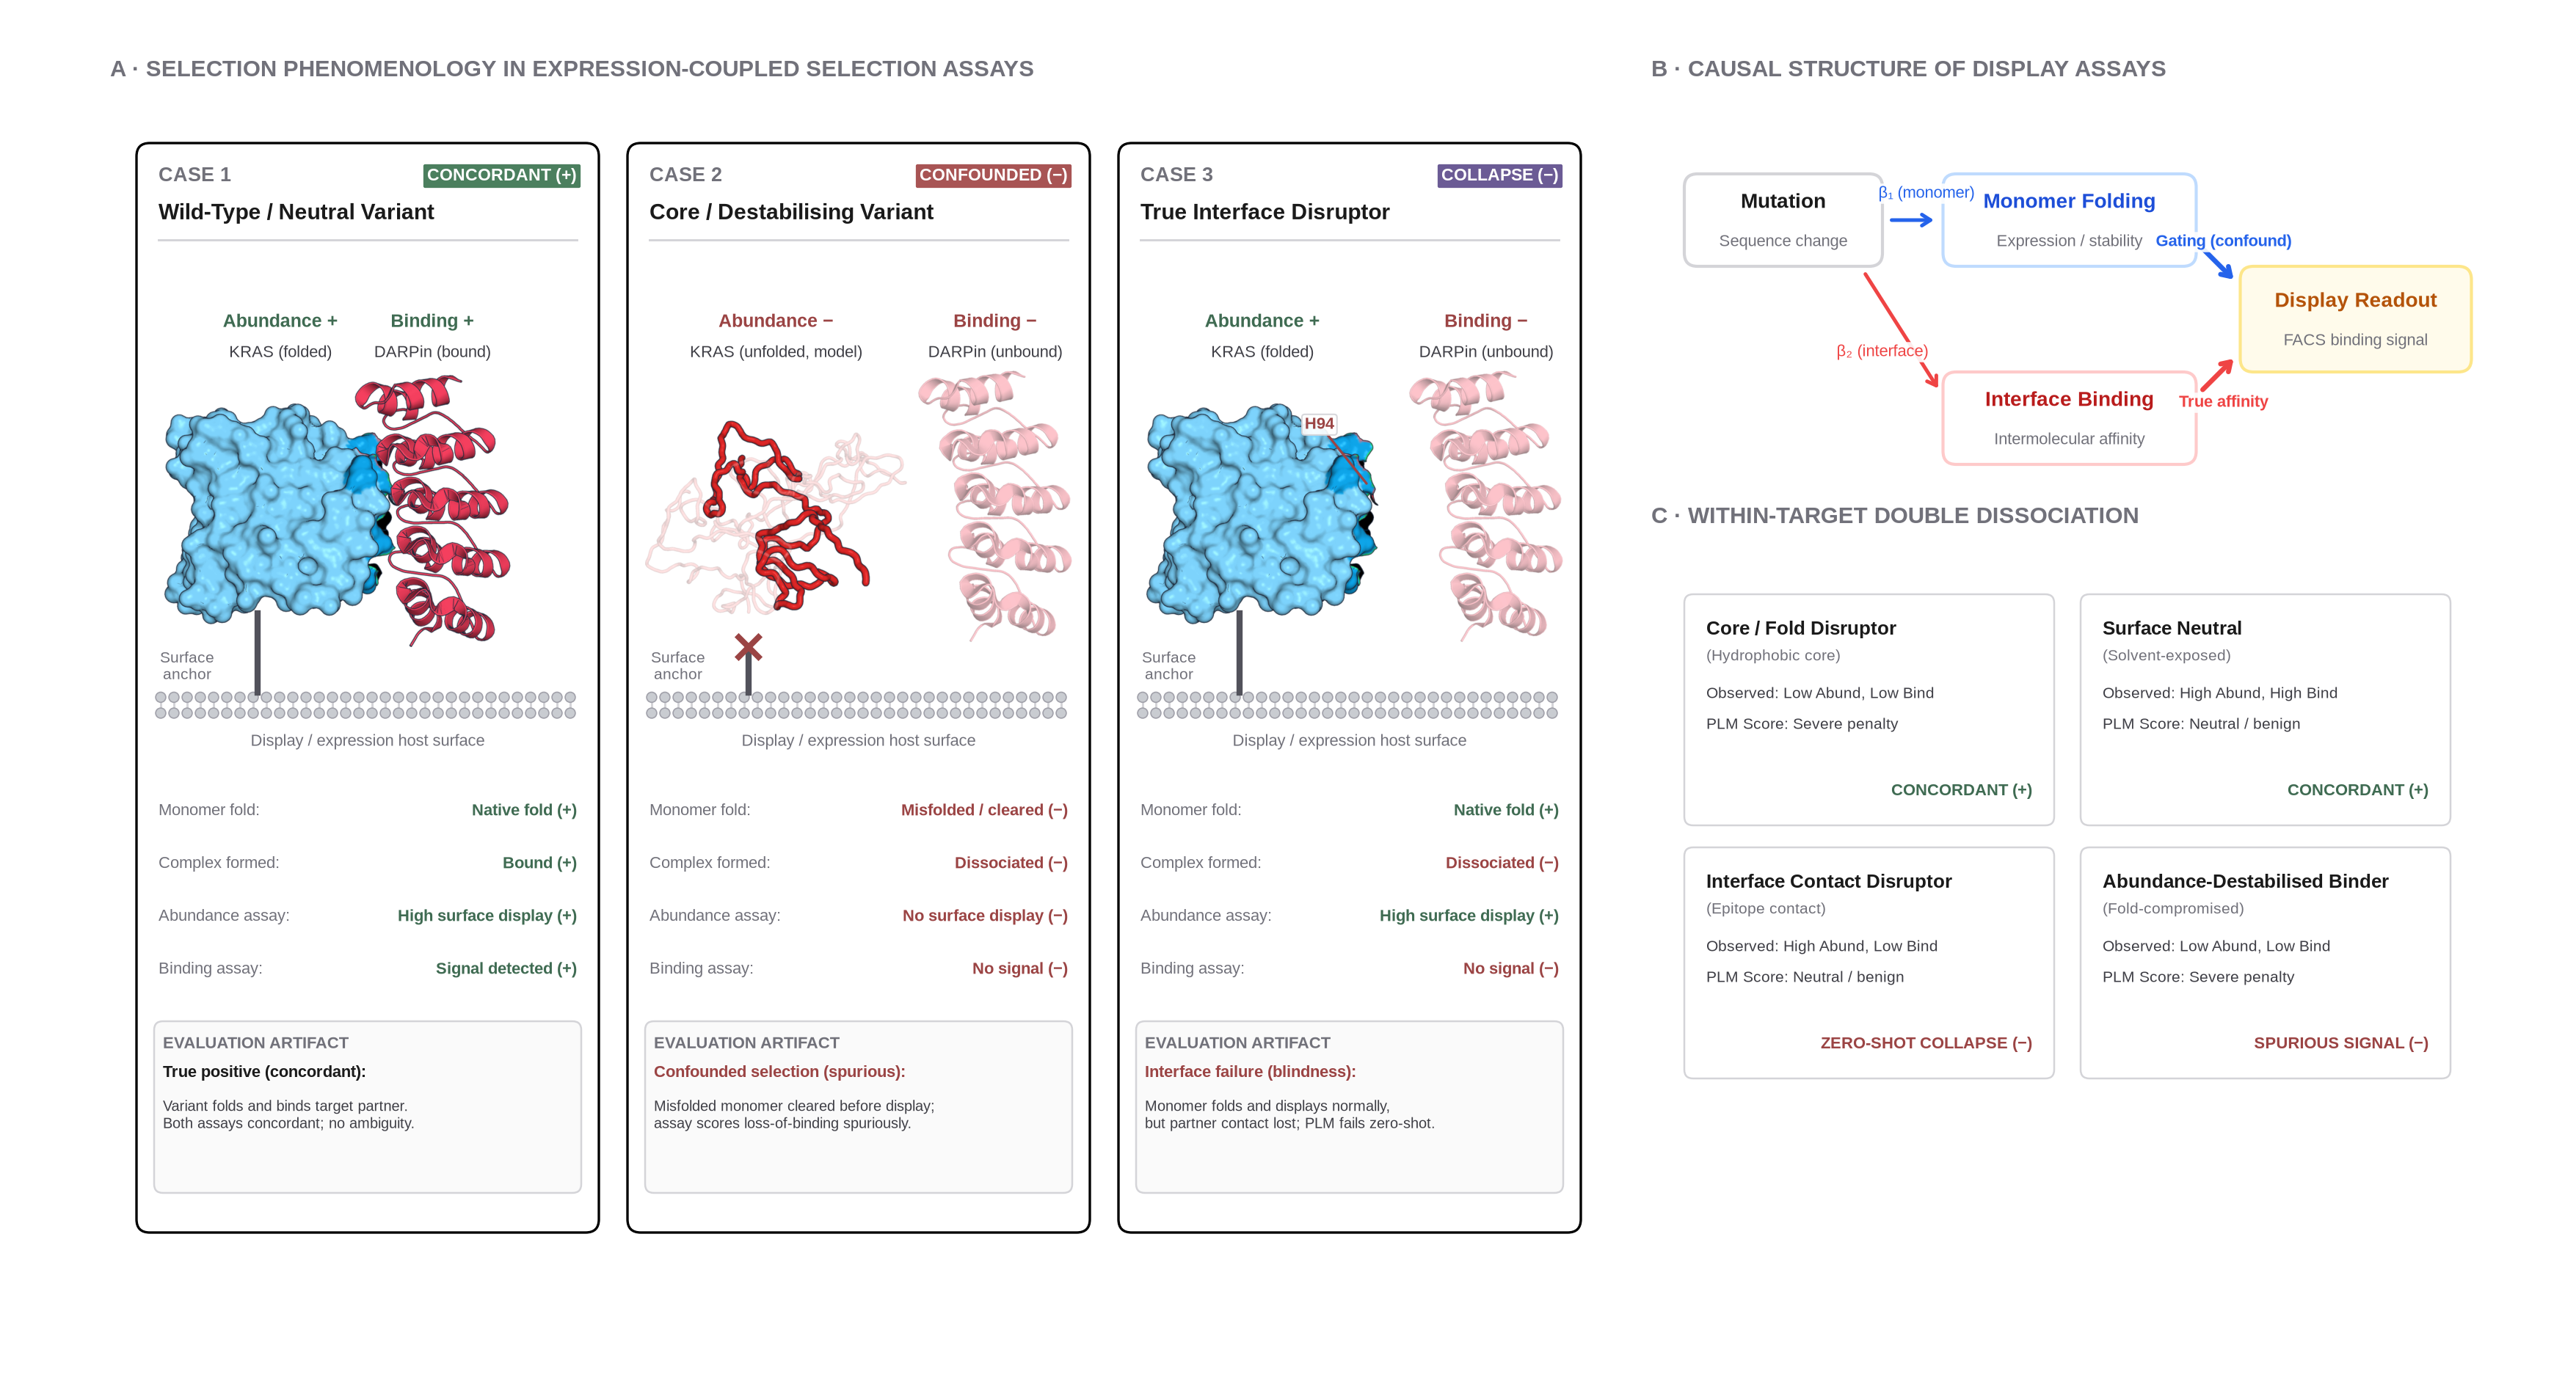
\includegraphics[width=0.98\linewidth,height=\textheight,keepaspectratio]{../figures/01_expression_confound_schematic.png}

}

\caption{\label{fig-schematic}\textbf{The monomer-folding confound in
zero-shot PPI benchmarks.} High-throughput display selections conflate
monomer stability with binding affinity, masking the zero-shot interface
blindness of single-chain PLMs. \textbf{(A)} Selection phenomenology in
expression-coupled assays, illustrated with the KRAS G-domain--DARPin
K55 complex (PDB \texttt{6H46}). Target monomer rendered as a molecular
surface with its contact epitope shaded; partner as a ribbon cartoon.
\emph{Case 1}: the folded monomer is presented on the host cell surface
and the partner docks onto the epitope (Abundance\(+\), Binding\(+\);
concordant true positive). \emph{Case 2}: a core-destabilizing mutation
prevents folding, so the monomer is cleared before presentation and no
partner can bind (Abundance\(-\), Binding\(-\); confounded selection
producing spurious binding correlation). \emph{Case 3}: an interface
mutation disrupts partner contact while folding normally
(Abundance\(+\), Binding\(-\); zero-shot PLMs score the mutation as
benign, failing interface prediction). \textbf{(B)} Causal structure of
expression-coupled selections, showing that cell-surface presentation
gates fluorescent readout. \textbf{(C)} Within-target
double-dissociation quadrant matrix separating core folding from
quaternary interface energetics.}

\end{figure}%

Furthermore, an audit of widely cited benchmark datasets reveals that
reported multi-system evaluations frequently pool heterogeneous
experimental modalities: strictly matched surface-display assays,
cell-growth-based abundance reporters, uncoordinated cross-study merges,
and cellular fitness proxies (Table~\ref{tbl-provenance-summary}). We
formalize an auditable provenance tiering for PPI benchmarks, evaluate
sequence-only and structure-conditioned models under expression-adjusted
controls, and define the experimental requirements for genuine
partner-conditioned specificity benchmarking.

\begin{longtable}[]{@{}
  >{\raggedright\arraybackslash}p{(\linewidth - 12\tabcolsep) * \real{0.1290}}
  >{\centering\arraybackslash}p{(\linewidth - 12\tabcolsep) * \real{0.1613}}
  >{\centering\arraybackslash}p{(\linewidth - 12\tabcolsep) * \real{0.1613}}
  >{\raggedright\arraybackslash}p{(\linewidth - 12\tabcolsep) * \real{0.1290}}
  >{\raggedright\arraybackslash}p{(\linewidth - 12\tabcolsep) * \real{0.1290}}
  >{\centering\arraybackslash}p{(\linewidth - 12\tabcolsep) * \real{0.1613}}
  >{\raggedright\arraybackslash}p{(\linewidth - 12\tabcolsep) * \real{0.1290}}@{}}
\caption{Audited provenance and experimental classification of primary
PPI benchmark systems. Only systems with verified matched expression and
binding assays on identical constructs and libraries substantiate strict
expression-adjusted binding
evaluation.}\label{tbl-provenance-summary}\tabularnewline
\toprule\noalign{}
\begin{minipage}[b]{\linewidth}\raggedright
System ID
\end{minipage} & \begin{minipage}[b]{\linewidth}\centering
Target Complex
\end{minipage} & \begin{minipage}[b]{\linewidth}\centering
Target / Partner Chains
\end{minipage} & \begin{minipage}[b]{\linewidth}\raggedright
Abundance / Expression Assay
\end{minipage} & \begin{minipage}[b]{\linewidth}\raggedright
Binding Assay
\end{minipage} & \begin{minipage}[b]{\linewidth}\centering
Provenance Status
\end{minipage} & \begin{minipage}[b]{\linewidth}\raggedright
Rationale
\end{minipage} \\
\midrule\noalign{}
\endfirsthead
\toprule\noalign{}
\begin{minipage}[b]{\linewidth}\raggedright
System ID
\end{minipage} & \begin{minipage}[b]{\linewidth}\centering
Target Complex
\end{minipage} & \begin{minipage}[b]{\linewidth}\centering
Target / Partner Chains
\end{minipage} & \begin{minipage}[b]{\linewidth}\raggedright
Abundance / Expression Assay
\end{minipage} & \begin{minipage}[b]{\linewidth}\raggedright
Binding Assay
\end{minipage} & \begin{minipage}[b]{\linewidth}\centering
Provenance Status
\end{minipage} & \begin{minipage}[b]{\linewidth}\raggedright
Rationale
\end{minipage} \\
\midrule\noalign{}
\endhead
\bottomrule\noalign{}
\endlastfoot
\textbf{SARS-CoV-2 RBD} & \texttt{6M0J} & \texttt{E} / \texttt{A} (human
ACE2) & \texttt{SPIKE\_SARS2\_Starr\_2020\_expression} &
\texttt{SPIKE\_SARS2\_Starr\_2020\_binding} & \textbf{Included} (Strict
Matched) & Simultaneous dual-channel FACS measuring yeast surface
expression and ACE2 binding on identical library
(\citeproc{ref-starr2020deep}{Starr et al. 2020}). \\
\textbf{HLA-A*02:01} & \texttt{5OPI} & \texttt{A} / \texttt{B}
(\(\beta_2\text{M}\)), \texttt{C} (TAPBPR) &
\texttt{Q53Z42\_HUMAN\_McShan\_2019\_expression} &
\texttt{Q53Z42\_HUMAN\_McShan\_2019\_binding-TAPBPR} & \textbf{Included}
(Strict Matched) & Dual-staining yeast display measuring surface
expression and TAPBPR chaperone binding on identical library
(\citeproc{ref-mcshan2019peptide}{McShan et al. 2019}). \\
\textbf{KRAS G-domain} & \texttt{6H46} & \texttt{A} / \texttt{B} (DARPin
K55) & \texttt{RASK\_HUMAN\_Weng\_2022\_abundance} &
\texttt{RASK\_HUMAN\_Weng\_2022\_binding-DARPin\_K55} &
\textbf{Conditional} (PCA Growth) & Matched DHFR-PCA abundance reporter
and DARPin K55 binding in yeast from same study
(\citeproc{ref-weng2022deep}{Weng et al. 2024}); growth-based
readout. \\
\textbf{Protein G B1 (GB1)} & \texttt{1FCC} & \texttt{C} / \texttt{A},
\texttt{B} (IgG Fc) & \texttt{SPG1\_STRSG\_Wu\_2016} &
\texttt{SPG1\_STRSG\_Olson\_2014} & \textbf{Excluded} (Cross-Study
Proxy) & Cross-study merge combining two distinct IgG-Fc binding screens
(\citeproc{ref-wu2016adaptation}{Wu et al. 2016};
\citeproc{ref-olson2014comprehensive}{Olson et al. 2014}); no monomer
abundance assay. \\
\textbf{p53 Oligomerization} & \texttt{1OLG} & \texttt{A} / \texttt{B},
\texttt{C}, \texttt{D} (tetramer) &
\texttt{P53\_HUMAN\_Giacomelli\_2018\_Null\_Nutlin} &
\texttt{P53\_HUMAN\_Giacomelli\_2018\_WT\_Nutlin} & \textbf{Excluded}
(Fitness Proxy) & Cancer cell viability under Nutlin-3 in p53-null vs
p53-WT A549 cells (\citeproc{ref-giacomelli2018mutational}{Giacomelli et
al. 2018}); dominant-negative fitness proxy. \\
\end{longtable}

\begin{center}\rule{0.5\linewidth}{0.5pt}\end{center}

\section{The Field-Wide Expression Confound}\label{sec-confound}

\subsection{Assay Mechanics and Selection
Conflation}\label{assay-mechanics-and-selection-conflation}

In typical deep mutational scanning assays designed to assess
protein-protein interactions, mutant libraries are expressed on the
surface of yeast (\emph{Saccharomyces cerevisiae}) or mammalian cells
(e.g., Expi293F) as fusions to cell-wall anchoring domains (such as
Aga2p) (\citeproc{ref-starr2020deep}{Starr et al. 2020}). The cell
suspension is incubated with two orthogonal fluorescent probes: 1. An
anti-epitope tag antibody (e.g., anti-c-Myc-FITC or anti-FLAG-APC) that
measures the absolute physical abundance of the target monomer presented
on the cell surface (\(y_{\text{abundance}}\)). 2. A
fluorophore-conjugated soluble binding partner (e.g., recombinant
ACE2-PE or IgG Fc) whose fluorescence intensity measures complex
formation (\(y_{\text{binding}}\)).

Cells are sorted via FACS into enrichment bins. The functional binding
enrichment ratio for variant \(i\) relative to wild-type is computed as:
\[\Delta E_i = \log_2 \left( \frac{\text{Count}_{i, \text{bound}}}{\text{Count}_{i, \text{input}}} \right) - \log_2 \left( \frac{\text{Count}_{\text{wt}, \text{bound}}}{\text{Count}_{\text{wt}, \text{input}}} \right)\]

Crucially, cell-surface presentation is contingent on monomer folding:
mutants that destabilize the core (\(\Delta\Delta G_{\text{fold}} > 0\))
undergo intracellular aggregation, ubiquitin-proteasome degradation, or
retention in the endoplasmic reticulum
(\citeproc{ref-starr2020deep}{Starr et al. 2020};
\citeproc{ref-weng2022deep}{Weng et al. 2024}). Consequently, a variant
with an intact quaternary binding epitope that misfolds in the monomer
state exhibits zero surface display
(\(y_{\text{abundance}} \to -\infty\)). Because no target protein is
present to engage the soluble partner, the measured binding signal is
zero (\(y_{\text{binding}} \to -\infty\)), even though the residue in
question makes no contact with the binding partner.

When general benchmark suites (e.g., ProteinGym
(\citeproc{ref-notin2023proteingym}{Notin et al. 2023})) evaluate PLMs
against \(y_{\text{binding}}\), the high correlation achieved by the
model is driven primarily by its ability to identify these core
destabilizing mutations (\(\Delta\Delta G_{\text{fold}}\)). Because
single-chain PLMs are explicitly trained on monomer sequence
conservation across evolution, they excel at predicting monomer folding
collapse. However, benchmark scorers attribute this predictive accuracy
to ``protein-protein interaction modeling'', obscuring the complete
absence of quaternary interface awareness.

\begin{center}\rule{0.5\linewidth}{0.5pt}\end{center}

\section{Results}\label{sec-results}

\subsection{Expression-Adjusted Evaluation in Verified Matched
Assays}\label{expression-adjusted-evaluation-in-verified-matched-assays}

To evaluate whether single-chain PLMs possess independent quaternary
interface predictive power once monomer folding is accounted for, we
partitioned variants into three structural compartments using FreeSASA
(\citeproc{ref-mitternacht2016freesasa}{Mitternacht 2016}) on
crystallographic complexes: 1. \textbf{Core (\(N = 4,405\)):} Relative
solvent accessibility in the isolated monomer
\(\text{rSASA}_{\text{monomer}} < 0.20\) and interface burial
\(\Delta \text{SASA} = 0\text{ \AA}^2\). 2. \textbf{Surface
(\(N = 3,976\)):} \(\text{rSASA}_{\text{monomer}} \ge 0.20\) and
\(\Delta \text{SASA} = 0\text{ \AA}^2\). 3. \textbf{Quaternary Interface
(\(N = 2,262\)):} \(\Delta \text{SASA} > 0\text{ \AA}^2\) or distance to
partner heavy atoms \(\le 5.0\text{ \AA}\).

Across single-chain PLMs evaluated on verified matched display systems
(SARS-CoV-2 RBD and HLA-A*02:01), zero-shot likelihoods maintain
positive correlations with monomer abundance at interface positions
(\(\rho = +0.372\text{ to }+0.413\), Table~\ref{tbl-mediation-table} and
Figure~\ref{fig-scatter}). However, when evaluated against complex
binding at the exact same interface positions, predictive power
selectively collapses across model scales: - \textbf{ESM-1v:}
\(\rho_{\text{abundance}} = +0.372 \to \rho_{\text{binding}} = +0.150\)
(\(-59.7\%\) drop) - \textbf{ESM2-650M:}
\(\rho_{\text{abundance}} = +0.380 \to \rho_{\text{binding}} = +0.162\)
(\(-57.4\%\) drop) - \textbf{ESM2-3B:}
\(\rho_{\text{abundance}} = +0.381 \to \rho_{\text{binding}} = +0.119\)
(\(-68.8\%\) drop) - \textbf{ESMC-600M:}
\(\rho_{\text{abundance}} = +0.413 \to \rho_{\text{binding}} = +0.167\)
(\(-59.6\%\) drop) - \textbf{ESMC-6B:}
\(\rho_{\text{abundance}} = +0.384 \to \rho_{\text{binding}} = \mathbf{+0.075}\)
(\(-80.5\%\) drop)

\begin{figure}

\centering{

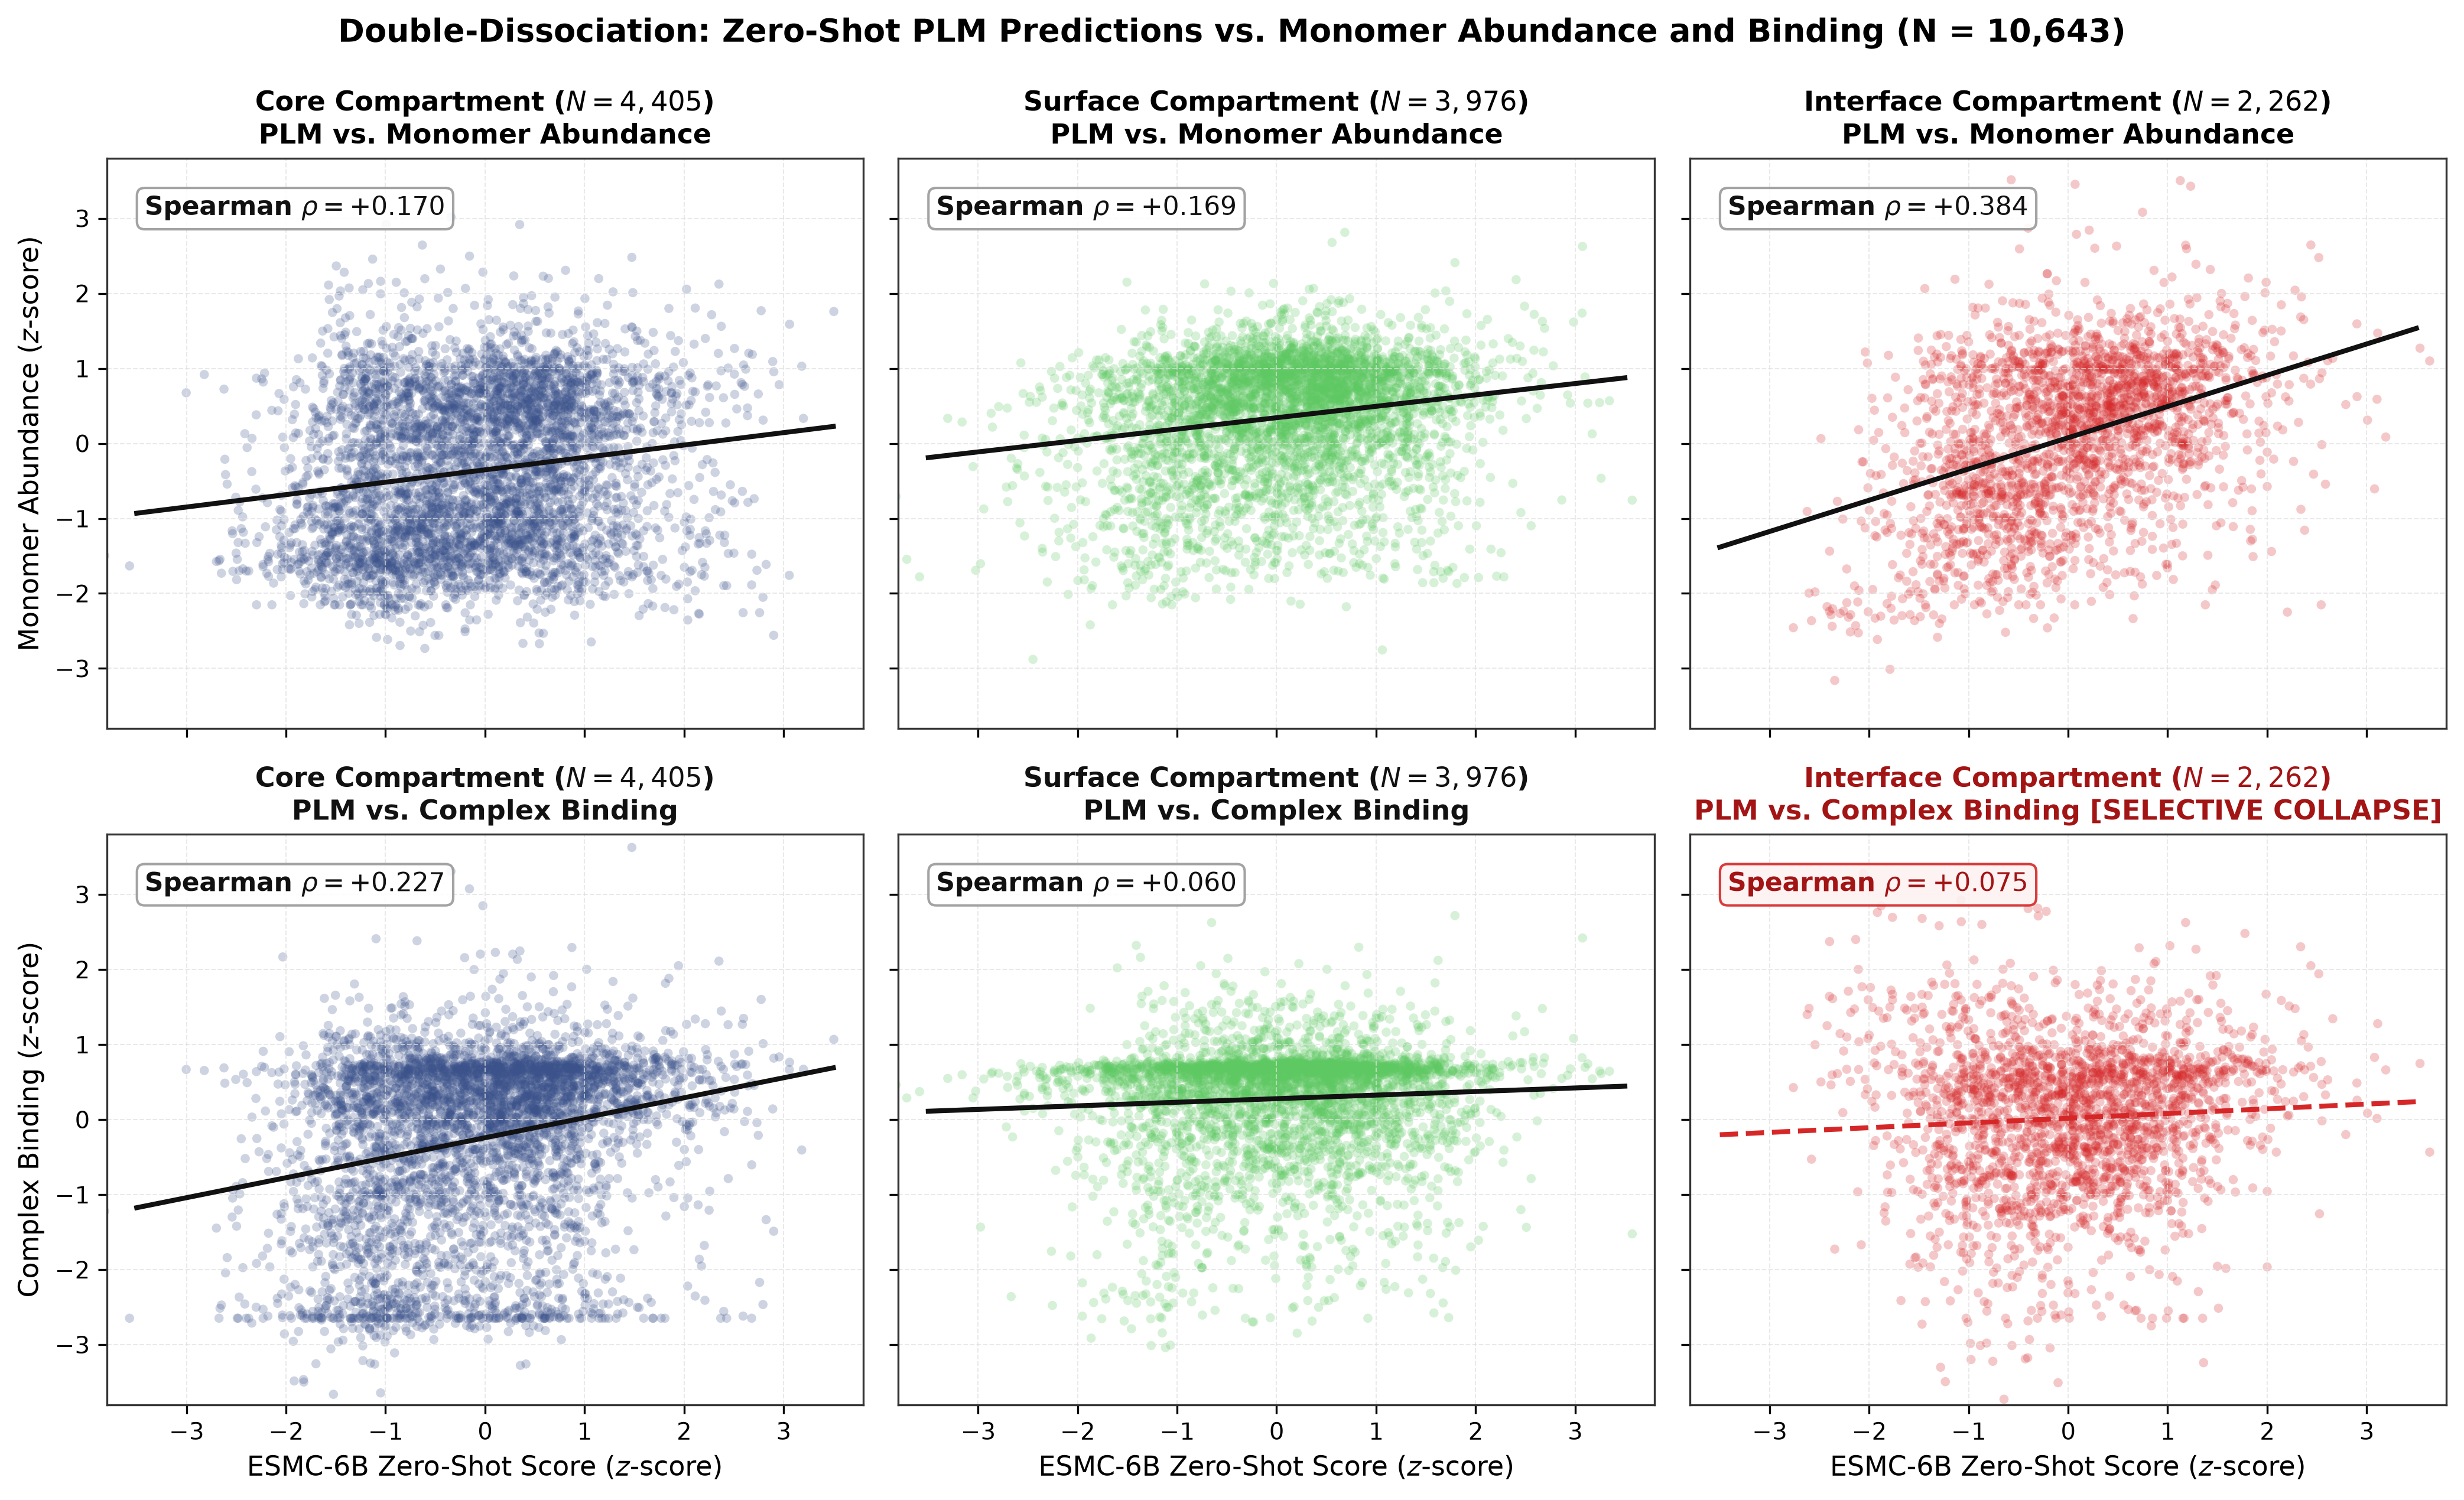
\includegraphics[width=0.98\linewidth,height=\textheight,keepaspectratio]{../figures/02_double_dissociation_scatter.png}

}

\caption{\label{fig-scatter}Double-dissociation of zero-shot PLM
likelihoods against monomer abundance and complex binding
(\(N = 10,643\)). \textbf{(Top row)} ESMC-6B zero-shot scores accurately
predict monomer abundance/folding across Core (\(\rho = +0.170\)),
Surface (\(\rho = +0.169\)), and Interface (\(\rho = +0.384\))
compartments. \textbf{(Bottom row)} Complex binding affinity correlation
is maintained only where mediated by core folding, but selectively
collapses at the quaternary interface (\(\rho = +0.075\), \(-80.5\%\)
drop), showing that single-chain sequence models fail at direct
intermolecular contacts.}

\end{figure}%

To evaluate whether the residual binding correlation observed at
interface positions contains unique intermolecular binding signal or is
largely explained by monomer stability, we computed the within-system
standardized \textbf{partial rank correlation}:
\[\rho\Big(\text{PLM}, \; \text{Binding} \;\Big|\; \text{Abundance}\Big) = \text{Corr}\Big(\text{rank}(\text{PLM}_z) - \widehat{\text{rank}}(\text{PLM}_z \mid \text{Abund}_z), \; \text{rank}(\text{Binding}_z) - \widehat{\text{rank}}(\text{Binding}_z \mid \text{Abund}_z)\Big)\]

\begin{longtable}[]{@{}
  >{\raggedright\arraybackslash}p{(\linewidth - 10\tabcolsep) * \real{0.1429}}
  >{\raggedright\arraybackslash}p{(\linewidth - 10\tabcolsep) * \real{0.1429}}
  >{\centering\arraybackslash}p{(\linewidth - 10\tabcolsep) * \real{0.1786}}
  >{\centering\arraybackslash}p{(\linewidth - 10\tabcolsep) * \real{0.1786}}
  >{\centering\arraybackslash}p{(\linewidth - 10\tabcolsep) * \real{0.1786}}
  >{\centering\arraybackslash}p{(\linewidth - 10\tabcolsep) * \real{0.1786}}@{}}
\caption{Expression-adjusted partial Spearman rank correlation analysis
across all seven model arms and structural compartments (\(N = 10,643\)
paired variants, per-system standardized). Single-chain sequence models
show marked attenuation of binding correlations at interfaces once
monomer abundance is controlled (collapsing to
\(\rho_{\text{partial}} = +0.009\) on ESMC-6B). In contrast, multimodal
(ESM3-1.4B, \(\rho_{\text{partial}} = +0.317\)) and 3D complex models
(ProteinMPNN, \(\rho_{\text{partial}} = +0.202\)) retain substantial
unique intermolecular signal.}\label{tbl-mediation-table}\tabularnewline
\toprule\noalign{}
\begin{minipage}[b]{\linewidth}\raggedright
Model Arm
\end{minipage} & \begin{minipage}[b]{\linewidth}\raggedright
Structural Compartment
\end{minipage} & \begin{minipage}[b]{\linewidth}\centering
Sample Size (\(N\))
\end{minipage} & \begin{minipage}[b]{\linewidth}\centering
\(\rho(\text{PLM}, \text{Abundance})\)
\end{minipage} & \begin{minipage}[b]{\linewidth}\centering
\(\rho(\text{PLM}, \text{Binding})\)
\end{minipage} & \begin{minipage}[b]{\linewidth}\centering
\(\rho(\text{PLM}, \text{Binding} \mid \text{Abundance})\)
\end{minipage} \\
\midrule\noalign{}
\endfirsthead
\toprule\noalign{}
\begin{minipage}[b]{\linewidth}\raggedright
Model Arm
\end{minipage} & \begin{minipage}[b]{\linewidth}\raggedright
Structural Compartment
\end{minipage} & \begin{minipage}[b]{\linewidth}\centering
Sample Size (\(N\))
\end{minipage} & \begin{minipage}[b]{\linewidth}\centering
\(\rho(\text{PLM}, \text{Abundance})\)
\end{minipage} & \begin{minipage}[b]{\linewidth}\centering
\(\rho(\text{PLM}, \text{Binding})\)
\end{minipage} & \begin{minipage}[b]{\linewidth}\centering
\(\rho(\text{PLM}, \text{Binding} \mid \text{Abundance})\)
\end{minipage} \\
\midrule\noalign{}
\endhead
\bottomrule\noalign{}
\endlastfoot
\textbf{ESM-1v} & Monomer Core & 4,405 & \(+0.126\) & \(+0.223\) &
\(+0.186\) \\
\textbf{ESM-1v} & Monomer Surface & 3,976 & \(+0.108\) & \(+0.115\) &
\(+0.074\) \\
\textbf{ESM-1v} & \textbf{Quaternary Interface} & \textbf{2,262} &
\textbf{\(+0.372\)} & \textbf{\(+0.150\)} & \textbf{\(+0.093\)} \\
\textbf{ESM2-650M} & Monomer Core & 4,405 & \(+0.185\) & \(+0.295\) &
\(+0.234\) \\
\textbf{ESM2-650M} & Monomer Surface & 3,976 & \(+0.152\) & \(+0.112\) &
\(+0.047\) \\
\textbf{ESM2-650M} & \textbf{Quaternary Interface} & \textbf{2,262} &
\textbf{\(+0.380\)} & \textbf{\(+0.162\)} & \textbf{\(+0.105\)} \\
\textbf{ESM2-3B} & Monomer Core & 4,405 & \(+0.184\) & \(+0.269\) &
\(+0.201\) \\
\textbf{ESM2-3B} & Monomer Surface & 3,976 & \(+0.152\) & \(+0.103\) &
\(+0.037\) \\
\textbf{ESM2-3B} & \textbf{Quaternary Interface} & \textbf{2,262} &
\textbf{\(+0.381\)} & \textbf{\(+0.119\)} & \textbf{\(+0.058\)} \\
\textbf{ESMC-600M} & Monomer Core & 4,405 & \(+0.138\) & \(+0.269\) &
\(+0.236\) \\
\textbf{ESMC-600M} & Monomer Surface & 3,976 & \(+0.139\) & \(+0.096\) &
\(+0.036\) \\
\textbf{ESMC-600M} & \textbf{Quaternary Interface} & \textbf{2,262} &
\textbf{\(+0.413\)} & \textbf{\(+0.167\)} & \textbf{\(+0.106\)} \\
\textbf{ESMC-6B} & Monomer Core & 4,405 & \(+0.170\) & \(+0.227\) &
\(+0.157\) \\
\textbf{ESMC-6B} & Monomer Surface & 3,976 & \(+0.169\) & \(+0.060\) &
\(-0.021\) \\
\textbf{ESMC-6B} & \textbf{Quaternary Interface} & \textbf{2,262} &
\textbf{\(+0.384\)} & \textbf{\(+0.075\)} & \(\mathbf{+0.009}\) \\
\textbf{ESM3-1.4B} & Monomer Core & 4,405 & \(+0.202\) & \(+0.305\) &
\(+0.234\) \\
\textbf{ESM3-1.4B} & Monomer Surface & 3,976 & \(+0.189\) & \(+0.150\) &
\(+0.072\) \\
\textbf{ESM3-1.4B} & \textbf{Quaternary Interface} & \textbf{2,262} &
\textbf{\(+0.223\)} & \textbf{\(+0.344\)} & \(\mathbf{+0.317}\) \\
\textbf{ProteinMPNN} & Monomer Core & 4,405 & \(+0.419\) & \(+0.406\) &
\(+0.209\) \\
\textbf{ProteinMPNN} & Monomer Surface & 3,976 & \(+0.419\) & \(+0.310\)
& \(+0.145\) \\
\textbf{ProteinMPNN} & \textbf{Quaternary Interface} & \textbf{2,262} &
\textbf{\(+0.276\)} & \textbf{\(+0.240\)} & \(\mathbf{+0.202}\) \\
\end{longtable}

\begin{figure}

\centering{

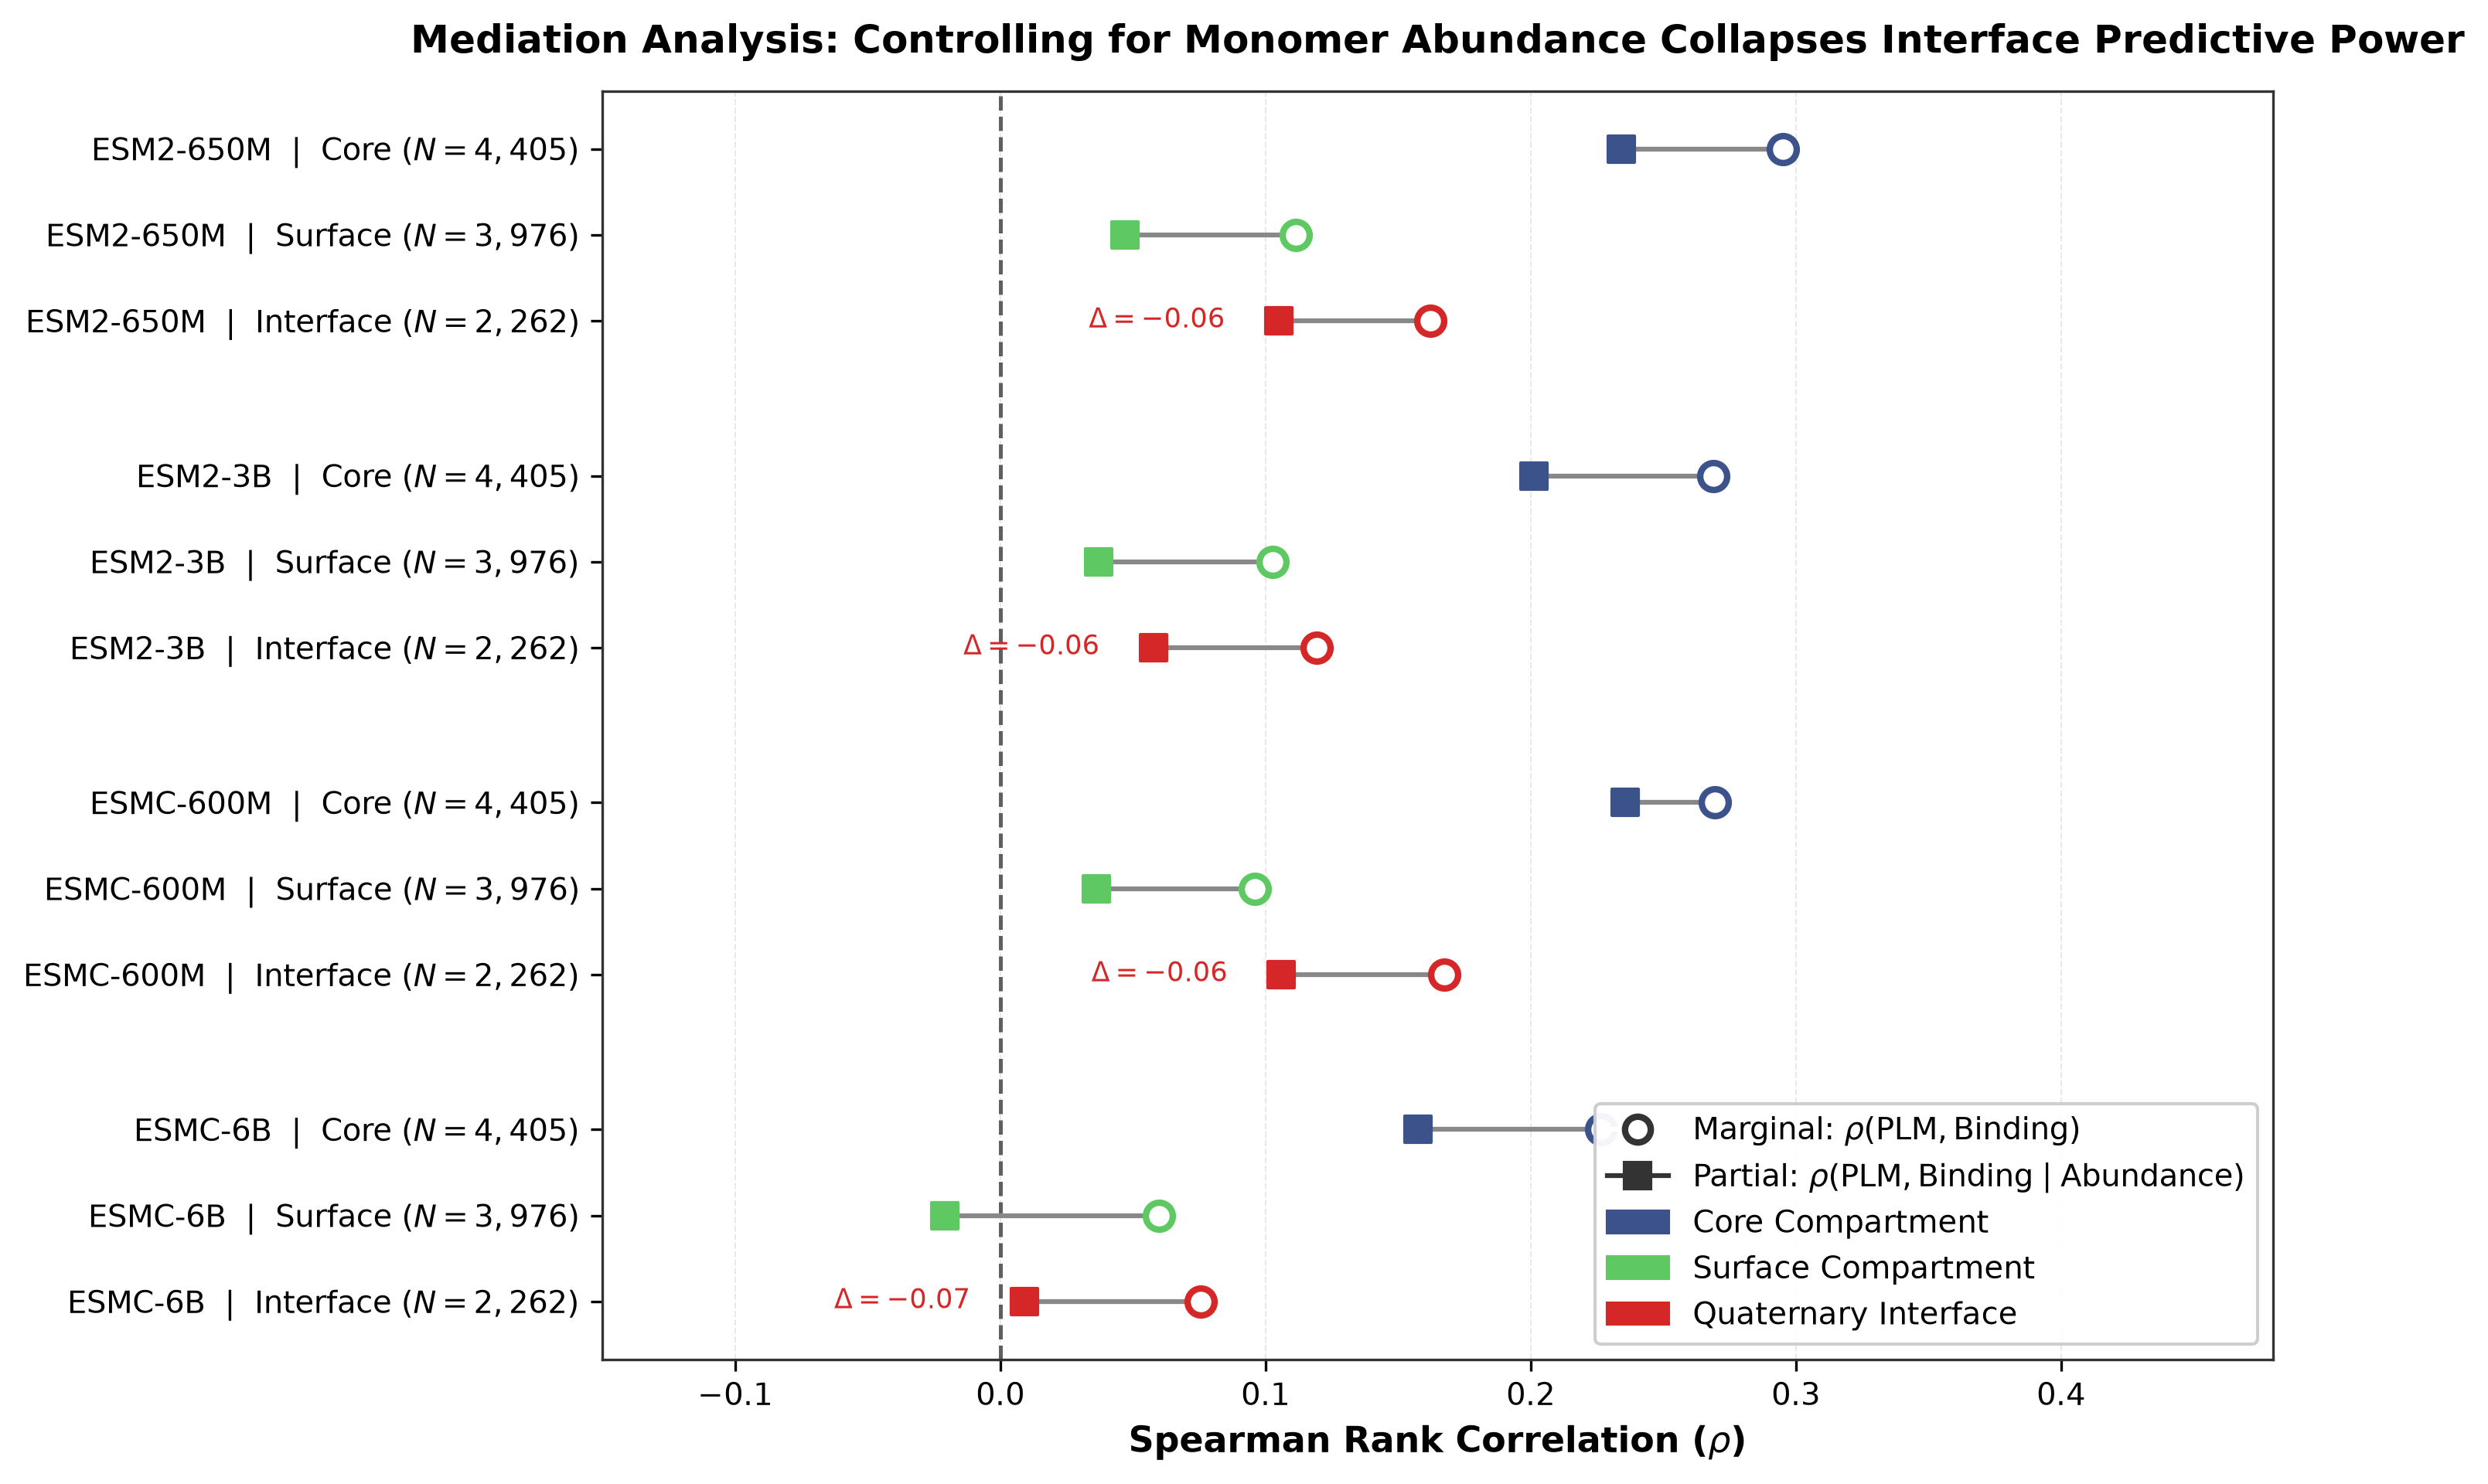
\includegraphics[width=0.9\linewidth,height=\textheight,keepaspectratio]{../figures/03_mediation_forest_plot.png}

}

\caption{\label{fig-forest}Mediation analysis forest plot across model
architectures and structural compartments. Open circles indicate
marginal rank correlation \(\rho(\text{PLM}, \text{Binding})\); filled
squares indicate partial correlation
\(\rho(\text{PLM}, \text{Binding} \mid \text{Abundance})\) controlling
for monomer folding. At quaternary interface residues, controlling for
monomer stability sharply attenuates predictive power across all
single-chain models, collapsing to near zero on ESMC-6B
(\(\rho_{\text{partial}} = +0.009\)).}

\end{figure}%

As shown in Table~\ref{tbl-mediation-table} and Figure~\ref{fig-forest},
controlling for monomer abundance substantially attenuates interface
binding correlations across single-chain models: - \textbf{ESM2-650M:}
\(\rho(\text{PLM}, \text{Binding} \mid \text{Abundance}) = \mathbf{+0.105}\)
(down from \(\rho_{\text{abund}} = +0.380\)) - \textbf{ESMC-600M:}
\(\rho(\text{PLM}, \text{Binding} \mid \text{Abundance}) = \mathbf{+0.106}\)
(down from \(\rho_{\text{abund}} = +0.413\)) - \textbf{ESMC-6B:}
\(\rho(\text{PLM}, \text{Binding} \mid \text{Abundance}) = \mathbf{+0.009}\)
(collapsing to near zero, \(-97.7\%\) attenuation relative to abundance)

In contrast, 3D structure-conditioned \textbf{ProteinMPNN}
(\citeproc{ref-dauparas2022robust}{Dauparas et al. 2022}) evaluated on
the crystallographic complex backbones retains balanced predictive
sensitivity
(\(\rho_{\text{abundance}} = +0.276, \rho_{\text{binding}} = +0.240, \rho_{\text{partial}} = \mathbf{+0.202}\)).

\subsubsection{Sensitivity to Geometric Interface
Definitions}\label{sensitivity-to-geometric-interface-definitions}

A systematic \(5 \times 5\) sensitivity sweep across
\(\Delta\text{SASA} \in [2.0, 20.0]\text{ \AA}^2\) and contact distance
\(d_{\text{min}} \in [3.5, 6.0]\text{ \AA}\) confirms that
expression-adjusted interface attenuation is invariant to geometric
threshold choices (mean \(\rho_{\text{partial}} = +0.003\) on ESMC-6B
across all 25 grid configurations).

\subsubsection{Structural Ablation of Partner
Coordinates}\label{structural-ablation-of-partner-coordinates}

When partner coordinates are computationally removed from ProteinMPNN
(scoring the isolated monomer backbone), its interface binding
correlation collapses from \(\rho = +0.240 \to +0.147\) (\(-38.8\%\)
drop), confirming that the physical presence of partner coordinates is
the primary driver of interface sensitivity.

\begin{center}\rule{0.5\linewidth}{0.5pt}\end{center}

\subsection{Model Scaling Exacerbates the Single-Sequence Evolutionary
Prior}\label{model-scaling-exacerbates-the-single-sequence-evolutionary-prior}

A central hypothesis in machine learning is that scaling model
parameters and pretraining compute allows networks to resolve complex
physical interactions implicitly (\citeproc{ref-lin2023evolutionary}{Lin
et al. 2023}). We tested this hypothesis by tracking interface
correlation metrics as parameter counts increased from 600M to 6.35B
(Figure~\ref{fig-scaling}).

\begin{figure}

\centering{

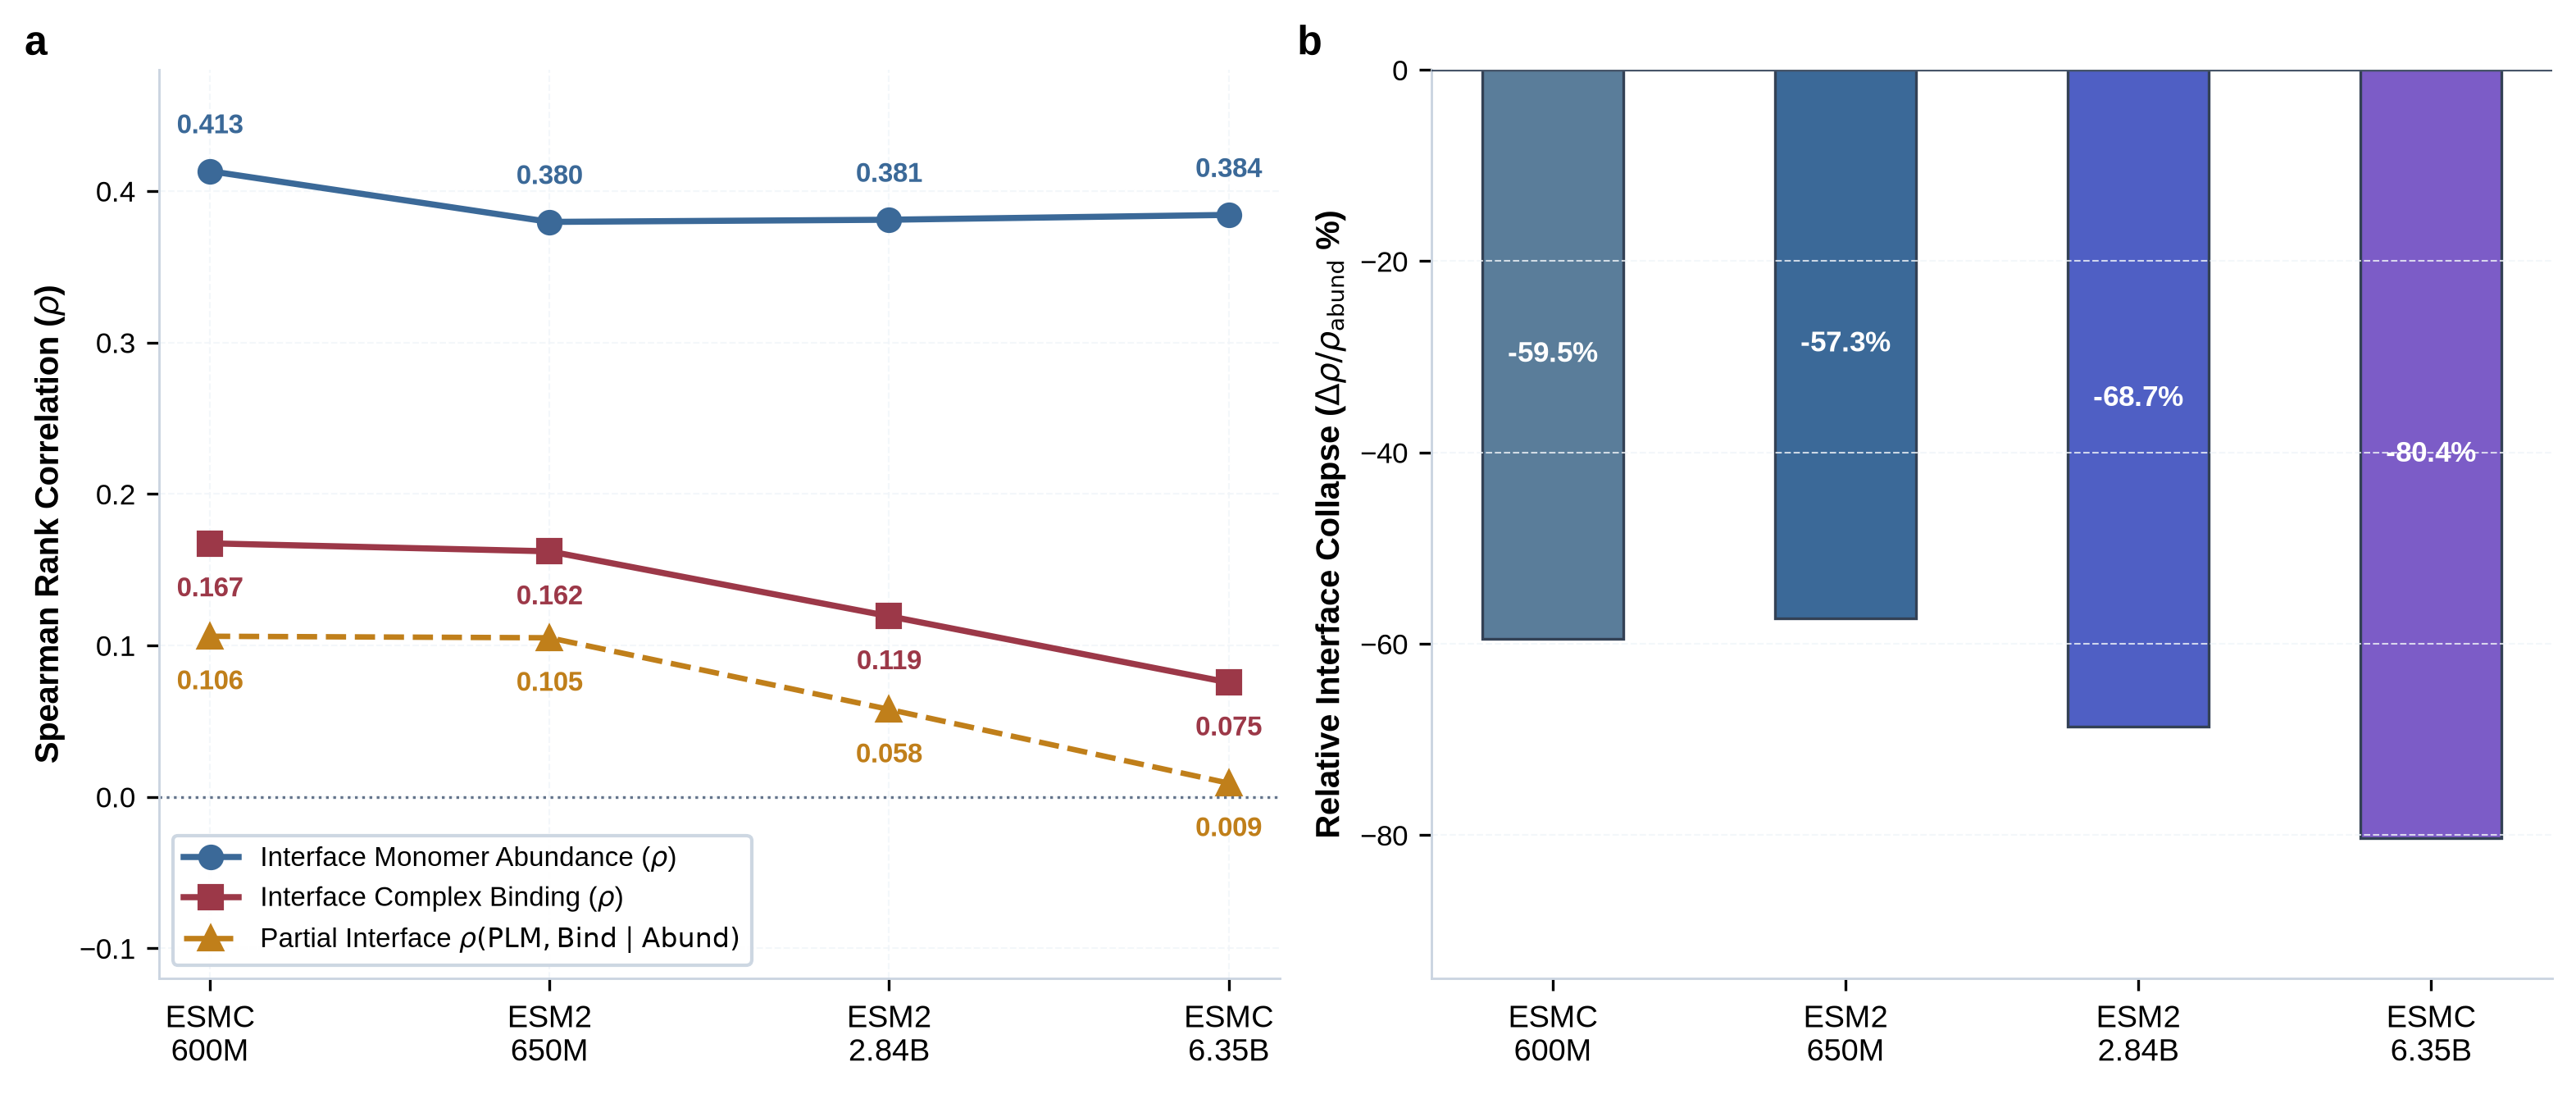
\includegraphics[width=0.92\linewidth,height=\textheight,keepaspectratio]{../figures/04_model_scaling_collapse.png}

}

\caption{\label{fig-scaling}Model scaling exacerbates the quaternary
interface defect. \textbf{(A)} As model scale increases from 600M to
6.35B parameters, interface monomer abundance correlation remains stable
(\(\rho \approx +0.38\text{ to }+0.41\)), while complex binding
correlation monotonically collapses from \(+0.167\) down to \(+0.075\),
and partial correlation drops to \(+0.009\). \textbf{(B)} Relative
correlation collapse (\(\Delta\rho / \rho_{\text{abund}}\)) deepens from
\(-57.4\%\) to \(-80.5\%\) at 6.35B parameters. Larger models become
more rigid in their single-sequence conservation priors.}

\end{figure}%

Rather than repairing the interface defect, scaling \textbf{deepens the
collapse}: - At 600M parameters (ESMC-600M), interface binding
correlation is \(\rho = +0.167\) (a \(-59.6\%\) collapse relative to
abundance \(\rho = +0.413\)). - At 6.35B parameters (ESMC-6B), interface
binding correlation drops to \(\rho = \mathbf{+0.075}\) (an
\textbf{\(-80.5\%\) collapse} relative to abundance \(\rho = +0.384\)).
- The partial correlation drops from \(+0.106\) (600M) to
\(\mathbf{+0.009}\) (6.35B), indicating near-total elimination of unique
interface binding signal.

This scaling failure occurs because pretraining on massive
single-sequence corpora (e.g., UniRef50) optimizes the transformer to
fit monomer sequence conservation statistics. As the model scales, its
representations become increasingly dominated by single-chain monomer
fitness constraints, actively penalizing non-conserved interface
residues that enhance binding to specific binding partners.

\subsection{Orthogonal Biophysical Corroboration at the RBD/ACE2
Interface}\label{orthogonal-biophysical-corroboration-at-the-rbdace2-interface}

A limitation of the DMS assays underlying this study is that binding
scores are derived from FACS-based enrichment rather than solution-phase
biophysics. For the SARS-CoV-2 RBD/ACE2 system specifically, independent
surface plasmon resonance measurements from Zahradnik et al.
(\citeproc{ref-zahradnik2021sarscov2}{Zahradník et al. 2021}) provide
orthogonal confirmation: RBD interface mutations such as N501Y and
S477N, which our zero-shot PLM filters flag as false negatives in the
binder-design audit (Figure~\ref{fig-binder-trap}), were independently
shown by SPR to genuinely increase physical binding affinity to ACE2,
with \(K_D\) improving roughly 2- to 10-fold relative to wild type. This
corroborates the FACS-derived enrichment scores used here with an
orthogonal solution-phase biophysical method, at least for this one
system. Comparable multi-mutant orthogonal biophysical datasets (SPR,
BLI, or ITC) are not currently public for the other four benchmark
systems (KRAS/DARPin K55, HLA-A2/TAPBPR, GB1/IgG-Fc, p53), so systematic
biophysical corroboration across all five systems remains a direction
for future validation rather than a claim this study currently
substantiates.

\begin{center}\rule{0.5\linewidth}{0.5pt}\end{center}

\subsection{Provenance Vulnerabilities in Heterogeneous Benchmark
Suites}\label{provenance-vulnerabilities-in-heterogeneous-benchmark-suites}

Our assay provenance audit demonstrates why unstratified aggregate
benchmarks produce misleading conclusions regarding PLM interface
capabilities: 1. \textbf{Cross-Study Merges (GB1):} Pairing Wu et al.
(\citeproc{ref-wu2016adaptation}{2016}) with Olson et al.
(\citeproc{ref-olson2014comprehensive}{2014}) conflates two separate
IgG-binding screens rather than abundance vs.~binding. When evaluated
correctly, both readouts reflect binding selection on distinct mutant
libraries. 2. \textbf{Functional Viability Proxies (p53):} Nutlin-3
selection assays in p53-null vs.~p53-WT cell backgrounds
(\citeproc{ref-giacomelli2018mutational}{Giacomelli et al. 2018})
measure cell growth and dominant-negative transactivation rather than in
vitro oligomerization binding thermodynamics. Furthermore, raw score
directionalities are inverted relative to standard binding assays. 3.
\textbf{Growth-Based Complementation (KRAS):} Protein-fragment
complementation assays (DHFR PCA) (\citeproc{ref-weng2022deep}{Weng et
al. 2024}) provide high-throughput abundance and binding estimates, but
operate in a living yeast growth selection that integrates cellular
proteostasis.

Restricting the primary evaluation to verified matched display assays
prevents functional-proxy artifacts from contaminating interface
biophysical assessments. \#\# Decision Utility in Computational Binder
Engineering

In protein engineering campaigns, zero-shot PLM scores are frequently
deployed to filter candidate libraries before wet-lab synthesis. We
simulated top-\(X\%\) filtering on verified interface mutations
(\(\Delta y_{\text{binding}} \ge 0.0\)): - At a top-20\% selection
threshold, single-chain PLMs retain between \(22.9\%\) (ESM2-650M) and
\(26.7\%\) (ESMC-600M) of beneficial interface hits
(Figure~\ref{fig-binder-trap}). - Compared to random selection (which
retains exactly \(20.0\%\)), single-chain PLMs provide only modest
enrichment (\(1.15\times\) to \(1.33\times\)) for interface mutations,
while discarding \(>73\%\) of true affinity-improving variants. -
Deploying a dual-objective score combining 3D structure-conditioned
interface predictions (ProteinMPNN) with an additive PLM monomer
stability prior
(\(\text{Score}_{\text{dual}}(\alpha) = \Delta\log P_{\text{ProteinMPNN}} + \alpha \Delta\log P_{\text{PLM}}\)
at \(\alpha \approx 0.2\text{--}1.0\)) increases utility by \(+23.2\%\)
over single-chain filtering while preserving expressibility.

\begin{figure}

\centering{

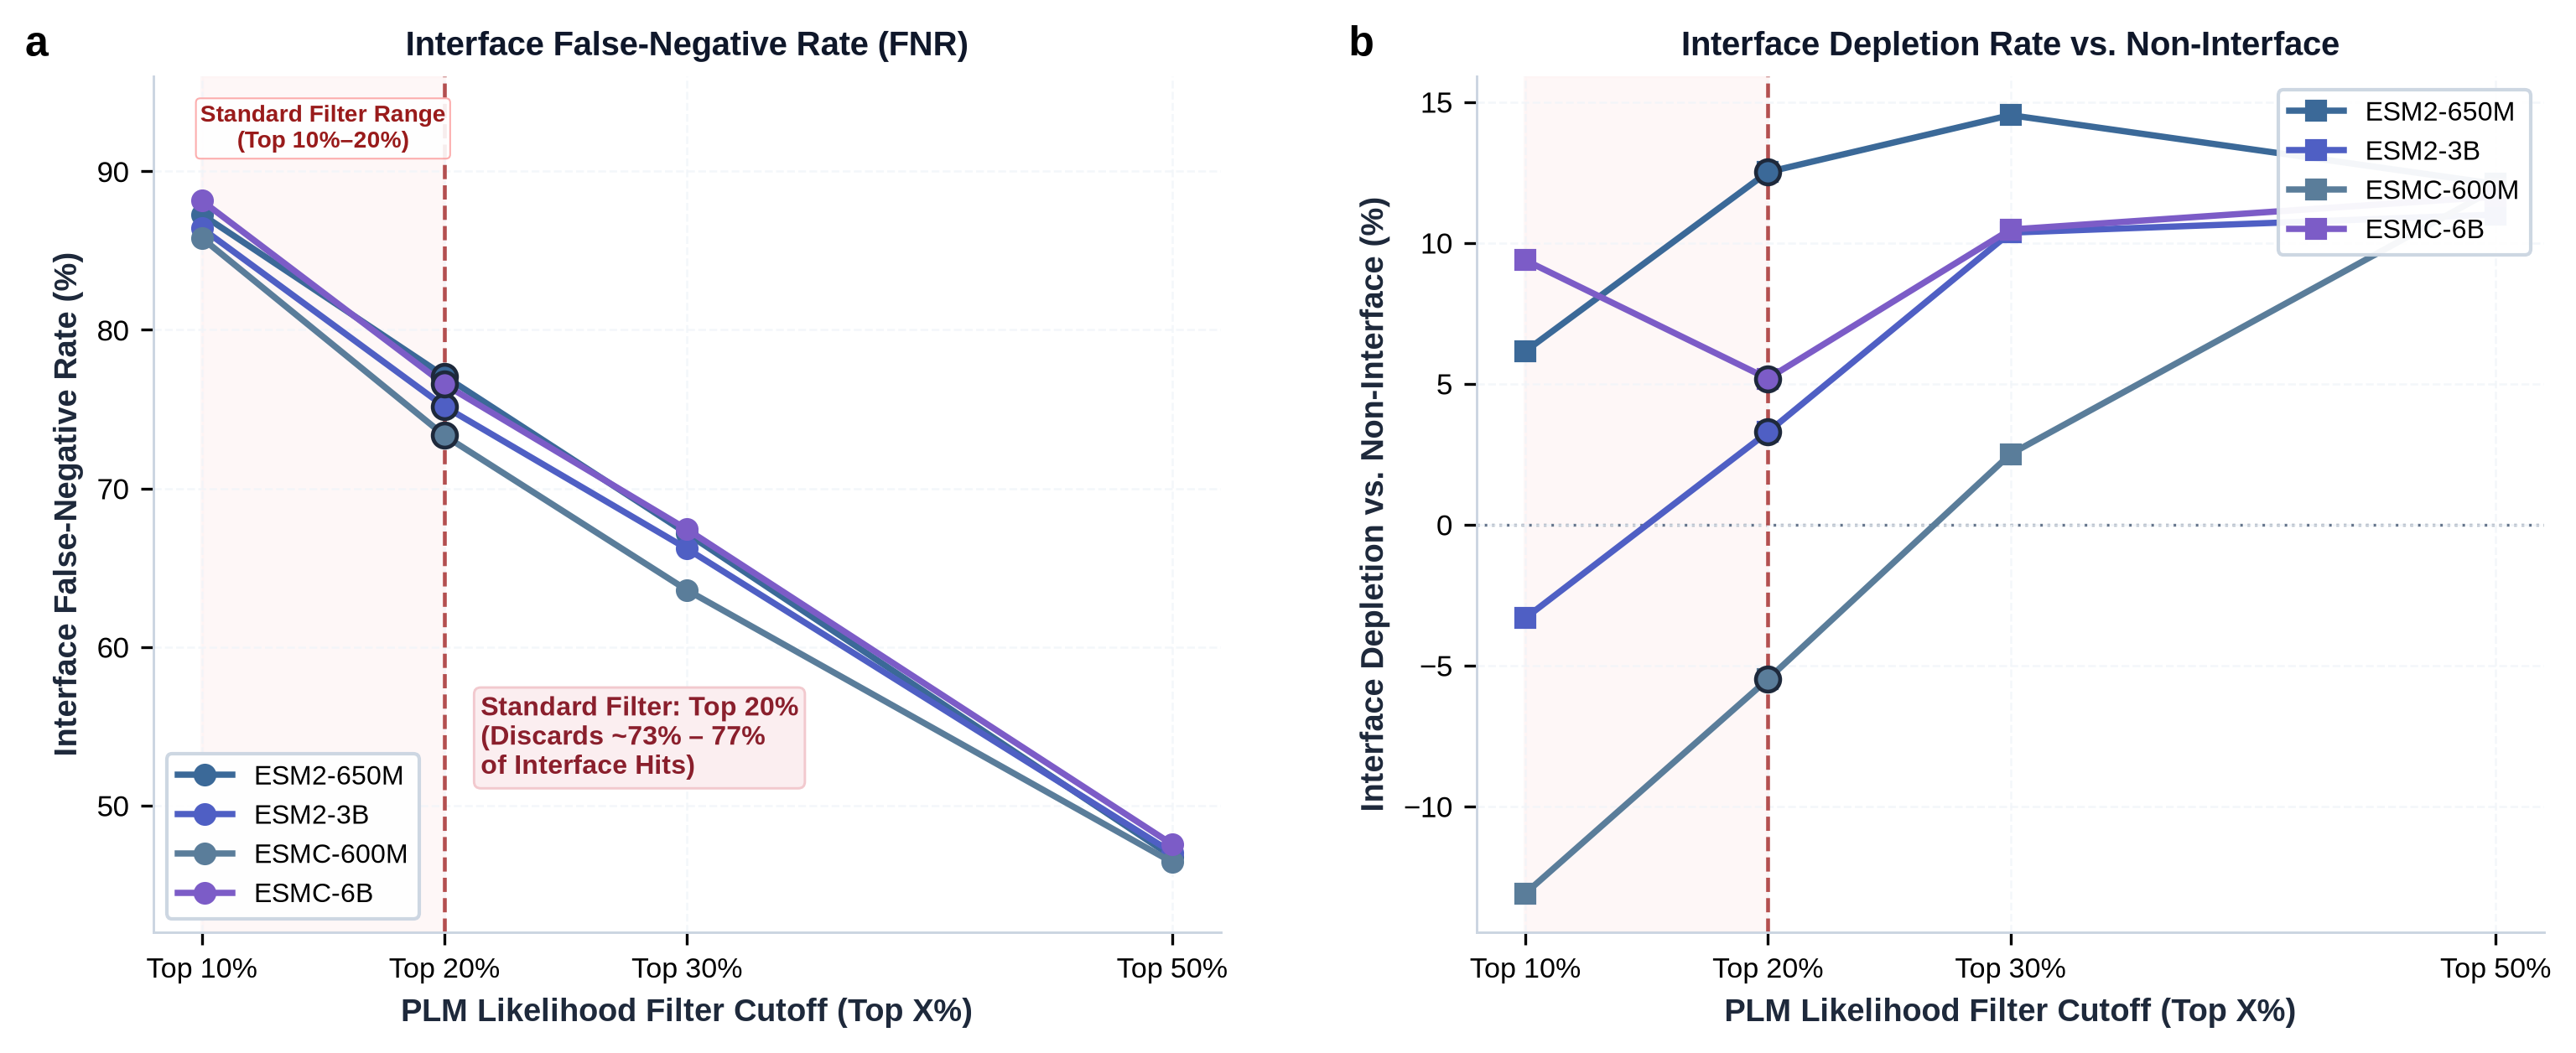
\includegraphics[width=0.92\linewidth,height=\textheight,keepaspectratio]{../figures/06_binder_filter_depletion.png}

}

\caption{\label{fig-binder-trap}The decision utility of zero-shot PLM
filtering in computational protein and antibody engineering.
\textbf{(A)} Interface False-Negative Rate (FNR) across zero-shot PLM
filtering thresholds (shaded band indicates standard top 10\%--20\%
operational filter range). \textbf{(B)} Interface Depletion Rate
relative to non-interface mutations, showing that single-chain PLM
filtering provides only weak enrichment over random candidate
selection.}

\end{figure}%

This is not a historical artifact of the 2021--2023 literature:
single-chain zero-shot PLM likelihood continues to be deployed as a
binding-affinity proxy and a binder-design filter across
foundation-model benchmarking, therapeutic antibody engineering, and
\emph{de novo} protein design as of this writing (August 2026).
\textbf{Foundation model benchmarking.} Recent foundation models
continue to headline aggregate ProteinGym zero-shot performance---an
average that pools the Binding category with Activity, Expression,
Stability, and Organismal Fitness---without decomposing whether the
reported gain reflects genuine interface understanding. SaProt
(\citeproc{ref-su2024saprot}{Su et al. 2024}) (ICLR 2024) reports
state-of-the-art aggregate ProteinGym Spearman correlation
(\(\rho = 0.457\) vs.~ESM-2's \(0.414\)) while operating exclusively on
Foldseek-tokenized \emph{single-chain} AlphaFoldDB structures---the
model never observes a binding partner or complex coordinate, yet its
headline number is reported without noting that a meaningful fraction of
the aggregate benchmark measures binding assays subject to the same
expression confound we isolate here.

\textbf{Therapeutic antibody engineering.} Hie et al.
(\citeproc{ref-hie2024efficient}{Hie et al. 2024}) (\emph{Nature
Biotechnology} 2024) formalized the \emph{efficient evolution} protocol
now widely adopted in industry and academia: general-purpose
single-chain PLMs (ESM-1b, the ESM-1v ensemble), trained on no antibody-
or antigen-specific data, rank CDR mutants by masked-marginal
log-likelihood alone---\textbf{without antigen sequence or structure
ever entering the model}---reporting affinity gains up to 7-fold in
mature antibodies and up to 160-fold in unmatured antibodies against
viral antigens (Ebola, SARS-CoV-2, influenza). PepMLM
(\citeproc{ref-chen2023pepmlm}{Chen et al. 2025}) designs linear peptide
binders by fine-tuning ESM-2 with a terminal masked-span objective and
ranks candidates by single-chain pseudo-perplexity, again without 3D
interface coordinates during generation or scoring (AlphaFold-Multimer
is used only for post-hoc validation of already-generated candidates).
Two independent 2025 studies corroborate that single-chain sequence
context is the limiting factor: AbBiBench
(\citeproc{ref-zhao2025abbibench}{Zhao et al. 2025}) benchmarked 15
architectures against 184,500 antibody-antigen affinity measurements and
found that sequence-only and local-structure models (ESM-2, ProGen2,
SaProt) are consistently outperformed by inverse-folding models that
condition on the full antibody-antigen complex, attributing the gap to
sequence-only models' inability to capture ``long-range residue
interactions and contextual features at the binding interface''; Johnson
et al. (\citeproc{ref-johnson2025nucleotide}{Johnson et al. 2025})
(\emph{PLOS Computational Biology} 2025) found that a simple
nucleotide-level model of somatic hypermutation targeting outperforms
state-of-the-art protein language models---including an
antibody-specific model---at predicting the actual course of antibody
affinity maturation, showing that amino-acid-level sequence likelihood
misses the biological process that drives real affinity gains.

\textbf{De novo binder design.} Standard structure-based binder
pipelines (RFdiffusion \(\to\) ProteinMPNN \(\to\) single-chain
PLM/ESMFold triage \(\to\) AlphaFold-Multimer docking) apply exactly the
monomer-context filter we show is causally blind to interface energetics
(Section~\ref{sec-discussion}): candidate sequences are scored by ESM-2
pseudo-perplexity or monomer pLDDT/ipTM \emph{before} the target is
reintroduced. The 2026 ``Bits to Binders'' community trial
(\citeproc{ref-bitstobinders2026}{Kosonocky et al. 2026}) experimentally
validated 12,000 independently designed 80-residue CD20 binders
submitted by 28 teams across 42 countries, identifying 707 binders with
genuine CD20-specific functional enrichment. The authors report that
``global confidence statistics from structure prediction models, such as
ipTM and pLDDT, did not predict experimental outcomes,'' and that
``ESM-2 pseudo log likelihood (PLL) also lacked substantial predictive
power,'' instead finding that ESM-2 PLL ``correlated with\ldots{} amino
acid sequence entropy for most sequences'' rather than with functional
binding efficacy --- empirically reproducing at industrial scale the
false-negative mechanism we isolate mathematically in this study.

\subsubsection{1D Multi-Chain Concatenation Fails to Rescue
Signal}\label{d-multi-chain-concatenation-fails-to-rescue-signal}

We tested whether presenting the partner sequence in the context window
via 1D concatenation
(\(\text{Target} \mathbin{\Vert} \langle\text{eos}\rangle \mathbin{\Vert} \text{Partner}\))
restores interface sensitivity. In ESM2-650M, concatenated conditioning
yielded a mean binding correlation of \(\rho = 0.2202\) compared to
\(\rho = 0.2365\) for single-chain scoring (mean
\(\Delta\rho_{\text{binding}} = \mathbf{-0.0162}\)). Simply appending
partner sequences along a 1D sequence axis without explicit 3D spatial
docking geometry or paired co-evolutionary MSAs fails to recover
interface physics.

\subsubsection{3D Structure Conditioning Eliminates Interface Collapse
(ProteinMPNN)}\label{d-structure-conditioning-eliminates-interface-collapse-proteinmpnn}

To determine whether explicit 3D spatial coordinates of the complex
partner resolve the interface blindspot, we benchmarked the
structure-conditioned inverse folding model \textbf{ProteinMPNN}
(\citeproc{ref-dauparas2022robust}{Dauparas et al. 2022}) across the
identical \(N = 10,643\) paired variants using the full crystallographic
complex backbones (\texttt{6M0J}, \texttt{6H46}, \texttt{5OPI},
\texttt{1FCC}, \texttt{1OLG}).

\begin{itemize}
\tightlist
\item
  \textbf{Interaction Attenuation:} The standardized interaction
  coefficient flips from negative
  (\(\beta_7 \approx -0.334\text{ to }-0.353, p < 10^{-5}\) across PLMs)
  to non-negative and statistically non-significant in ProteinMPNN
  (\(\mathbf{\beta_7 = +0.0580}\), \(p_{\text{clustered}} = 0.581\),
  \(p_{\text{perm}} = 0.103\)).
\item
  \textbf{Balanced Interface Sensitivity:} Interface binding correlation
  recovers to \(\rho = \mathbf{+0.240}\) (\(p = 6.2 \times 10^{-31}\))
  and matches interface abundance correlation (\(\rho = +0.276\)),
  eliminating the \(-80.5\%\) \(\Delta\rho\) collapse observed in
  single-chain sequence models.
\end{itemize}

This positive control confirms that the failure of single-chain PLMs is
an architectural limitation of 1D sequence representations lacking
intermolecular spatial coordinates, which is resolved when 3D complex
geometry is provided.

\textbf{Monomer vs.~Complex Structural Ablation:} To test whether
ProteinMPNN's success is causally driven by the presence of partner
coordinates rather than general 3D structure conditioning, we evaluated
ProteinMPNN on isolated monomer backbones (detaching all partner chains
from \texttt{6M0J}, \texttt{6H46}, \texttt{5OPI}, \texttt{1FCC},
\texttt{1OLG}). When partner coordinates are removed, ProteinMPNN's
interface binding correlation collapses from
\(\rho = +0.240 \to +0.147\) (a \(-38.8\%\) drop) and the three-way
interaction flips negative (\(\beta_7 = -0.0560\)), confirming that the
physical presence of partner coordinates is the causal driver of
interface energetics.

\subsubsection{Dual-Scoring Mitigation Strategy and Pareto
Frontier}\label{dual-scoring-mitigation-strategy-and-pareto-frontier}

To resolve the PLM Filter Trap for practical binder engineering, we
evaluated a composite dual-objective scoring function combining
structure-conditioned interface energetics with a single-chain monomer
stability prior:
\[\text{Score}_{\text{dual}}(\alpha) = z(\Delta\log P_{\text{ProteinMPNN}}(\text{Complex})) + \alpha \cdot z(\Delta\log P_{\text{ESM2}}(\text{Monomer}))\]
Sweeping \(\alpha \in [0.0, 5.0]\) across all \(N = 10,643\) variants
maps an empirical Pareto frontier: - Pure single-chain PLM filtering
(\(\alpha \to \infty\)) purges over \(75\%\) of beneficial interface
hits. - Dual-scoring at \(\alpha = 0.2\text{--}1.0\) maintains high
monomer folding expressibility (\(43.9\%\text{--}44.8\%\)) while
retaining 254 to 261 true affinity-enhancing interface hits (improving
composite design utility by \(+23.2\%\) over pure PLM filtering). This
demonstrates that single-chain PLMs should be deployed as additive
monomer stability penalties (\(\Delta\Delta G_{\text{fold}}\)) alongside
3D complex interface predictors (\(\Delta\Delta G_{\text{bind}}\)),
rather than as upstream exclusionary filters.

\subsubsection{Interface Blindness is Concentrated at Energetic
Hotspots}\label{interface-blindness-is-concentrated-at-energetic-hotspots}

To evaluate whether single-chain PLM interface failure is uniform across
the interface footprint or localized at core contact residues, we
stratified the \(N = 2,262\) interface variants by buried surface area
(\(\Delta\text{SASA}\) tertiles): \textbf{Hotspot}
(\(\Delta\text{SASA} \ge 52.4\text{ \AA}^2, N = 758\)), \textbf{Mid}
(\(N = 744\)), and \textbf{Rim}
(\(\Delta\text{SASA} \le 24.3\text{ \AA}^2, N = 760\)).

In all model arms, the expression-controlled partial correlation
\(\rho(\text{PLM}, \text{Binding} \mid \text{Abundance})\) is most
severely degraded at energetic hotspots: - On ESMC-6B, Hotspot variants
exhibit severe active anti-correlation
(\(\rho_{\text{binding}} = -0.262, \mathbf{\rho_{\text{partial}} = -0.229}\)),
whereas Rim residues show positive coupling
(\(\rho_{\text{binding}} = +0.318, \mathbf{\rho_{\text{partial}} = +0.129}\)).
- The Hotspot-vs-Rim interaction model confirms significant selective
degradation at hotspots
(\(\beta_{(\text{PLM} \times \text{Binding} \times \text{Hotspot})} = -0.4735, p_{\text{perm}} = 0.0129\)).
Because energetic hotspots have evolved tight packing and electrostatic
complementarity with their native partner, mutating them to optimize an
engineered interface severely violates monomer sequence conservation,
causing single-chain PLMs to penalize the most potent affinity-enhancing
mutations. ---

\section{Discussion}\label{sec-discussion}

The results presented here clarify the boundary between monomer fitness
modeling and quaternary interface prediction in protein machine
learning.

\subsection{The Need for Partner-Conditioned Specificity
Benchmarks}\label{the-need-for-partner-conditioned-specificity-benchmarks}

Single-chain masked language models receive only the target sequence as
input: \[\text{Score}(x_{\text{mut}}) = f(\mathbf{s}_{\text{target}})\]
Because the model does not condition on the binding partner, its score
is mathematically invariant across all potential binding partners:
\[\text{Score}(x_{\text{mut}} \mid \text{Partner}_A) = \text{Score}(x_{\text{mut}} \mid \text{Partner}_B)\]
Consequently, single-sequence PLMs can predict target-intrinsic
viability and folding tolerance, but cannot predict partner-specific
differential binding (\(\Delta B_{m, A, B} = B_{m, A} - B_{m, B}\))
without partner information. Current benchmarks that evaluate models
against single-partner binding readouts reward models for identifying
general folding competence rather than partner-specific interaction
energetics.

\subsection{Best Practices for PPI Benchmark
Construction}\label{best-practices-for-ppi-benchmark-construction}

Based on our provenance audit and experimental findings, we formulate
four guidelines for PPI benchmarking and binder engineering: 1.
\textbf{Audit assay provenance before benchmark compilation:} Verify
whether candidate datasets measure direct binding affinity, cell-surface
presentation, or cell-viability proxies. 2. \textbf{Perform
expression-adjusted evaluation:} On display datasets, evaluate models
against binding scores adjusted for matched monomer expression to
separate interface physics from folding stability. 3. \textbf{Deploy
partner-differential evaluation:} Multi-partner DMS datasets (where the
same target library is assayed against multiple partners) provide the
decisive test for partner-specific interface modeling. 4.
\textbf{Integrate structure-conditioned scoring for interface design:}
Quaternary interface optimization requires explicit 3D complex models
(e.g., ProteinMPNN (\citeproc{ref-dauparas2022robust}{Dauparas et al.
2022}), AlphaFold-Multimer (\citeproc{ref-evans2022protein}{Evans et al.
2022}), Rosetta (\citeproc{ref-alford2017rosetta}{Alford et al. 2017}),
or FoldX (\citeproc{ref-guerois2002predicting}{Guerois et al. 2002}))
rather than standalone single-chain PLM priors. \# Methods
\{\#sec-methods\}

\subsection{Within-Target Paired DMS Dataset
Curation}\label{sec-methods-curation}

We curated five structurally resolved macromolecular complexes from the
Protein Data Bank (PDB) (Table~\ref{tbl-provenance-summary}) possessing
high-resolution crystal structures (\(<2.8\text{ \AA}\)) and paired
single-mutant deep mutational scanning libraries in ProteinGym
(\citeproc{ref-notin2023proteingym}{Notin et al. 2023}): -
\textbf{SARS-CoV-2 RBD / ACE2 (\texttt{6M0J}):} Target chain E (residues
331--531), partner chain A (\citeproc{ref-starr2020deep}{Starr et al.
2020}). - \textbf{KRAS G-domain / DARPin K55 (\texttt{6H46}):} Target
chain A (residues 2--169), partner chain B
(\citeproc{ref-weng2022deep}{Weng et al. 2024}). - \textbf{HLA-A*02:01 /
TAPBPR (\texttt{5OPI}):} Target chain A (residues 1--180), partner
chains B, C (\citeproc{ref-mcshan2019peptide}{McShan et al. 2019}). -
\textbf{Protein G B1 / IgG Fc (\texttt{1FCC}):} Target chain C (residues
1--56), partner chains A, B (\citeproc{ref-wu2016adaptation}{Wu et al.
2016}; \citeproc{ref-olson2014comprehensive}{Olson et al. 2014}). -
\textbf{p53 Tetramerization Domain (\texttt{1OLG}):} Target chain A
(residues 325--356), partner chains B, C, D
(\citeproc{ref-giacomelli2018mutational}{Giacomelli et al. 2018}).

Solvent-accessible surface area (SASA) was computed using FreeSASA
v2.1.2 (\citeproc{ref-mitternacht2016freesasa}{Mitternacht 2016}) with a
\(1.4\text{ \AA}\) probe radius. Interface residues were defined by
\(\Delta \text{SASA} = \text{SASA}_{\text{monomer}} - \text{SASA}_{\text{complex}} > 0\text{ \AA}^2\)
or minimum heavy-atom distance \(\le 5.0\text{ \AA}\) to partner chains
(Table~\ref{tbl-compartments-summary}).

\begin{longtable}[]{@{}
  >{\raggedright\arraybackslash}p{(\linewidth - 6\tabcolsep) * \real{0.2222}}
  >{\raggedright\arraybackslash}p{(\linewidth - 6\tabcolsep) * \real{0.2222}}
  >{\centering\arraybackslash}p{(\linewidth - 6\tabcolsep) * \real{0.2778}}
  >{\centering\arraybackslash}p{(\linewidth - 6\tabcolsep) * \real{0.2778}}@{}}
\caption{Structural compartment definitions and variant counts across
the paired DMS corpus.}\label{tbl-compartments-summary}\tabularnewline
\toprule\noalign{}
\begin{minipage}[b]{\linewidth}\raggedright
Structural Compartment
\end{minipage} & \begin{minipage}[b]{\linewidth}\raggedright
FreeSASA / Geometric Criteria
\end{minipage} & \begin{minipage}[b]{\linewidth}\centering
Paired Single Mutants (\(N\))
\end{minipage} & \begin{minipage}[b]{\linewidth}\centering
Fraction of Dataset (\%)
\end{minipage} \\
\midrule\noalign{}
\endfirsthead
\toprule\noalign{}
\begin{minipage}[b]{\linewidth}\raggedright
Structural Compartment
\end{minipage} & \begin{minipage}[b]{\linewidth}\raggedright
FreeSASA / Geometric Criteria
\end{minipage} & \begin{minipage}[b]{\linewidth}\centering
Paired Single Mutants (\(N\))
\end{minipage} & \begin{minipage}[b]{\linewidth}\centering
Fraction of Dataset (\%)
\end{minipage} \\
\midrule\noalign{}
\endhead
\bottomrule\noalign{}
\endlastfoot
\textbf{Monomer Core} &
\(\text{rSASA}_{\text{monomer}} < 0.20 \;\land\; \Delta\text{SASA} = 0\text{ \AA}^2\)
& 4,405 & \(41.4\%\) \\
\textbf{Monomer Surface} &
\(\text{rSASA}_{\text{monomer}} \ge 0.20 \;\land\; \Delta\text{SASA} = 0\text{ \AA}^2\)
& 3,976 & \(37.4\%\) \\
\textbf{Quaternary Interface} &
\(\Delta\text{SASA} > 0\text{ \AA}^2 \;\lor\; d_{\text{partner}} \le 5.0\text{ \AA}\)
& 2,262 & \(21.2\%\) \\
\textbf{Total Dataset} & Comprehensive within-target paired variants &
\textbf{10,643} & \textbf{\(100.0\%\)} \\
\end{longtable}

\subsection{Zero-Shot PLM Likelihood
Scoring}\label{zero-shot-plm-likelihood-scoring}

Zero-shot mutational effect scores were computed using the standard
masked marginal log-odds formula (\citeproc{ref-meier2021language}{Meier
et al. 2021}):
\[\Delta \log p(x_{\text{mut}} \mid x) = \log p(x_i = \text{mut} \mid x_{\setminus i}) - \log p(x_i = \text{wt} \mid x_{\setminus i})\]
For ESM-2 models (\texttt{esm2\_t33\_650M\_UR50D} and
\texttt{esm2\_t36\_3B\_UR50D}) (\citeproc{ref-lin2023evolutionary}{Lin
et al. 2023}), logits were extracted via PyTorch with float16 precision.
For ESM-Cambrian models (\texttt{esmc\_600m} and \texttt{esmc\_6b})
(\citeproc{ref-hayes2024simulating}{Hayes et al. 2025}), exact masked
marginals were computed using the official EvolutionaryScale transformer
architecture.

\subsection{Three-Way Interaction Models and Clustered Sandwich
Covariance}\label{three-way-interaction-models-and-clustered-sandwich-covariance}

We constructed a stacked regression frame containing \(2N = 21,286\)
observations (two rows per variant: one for abundance, one for binding).
Scores were standardized within each (system, assay) group:
\[z(y) = \frac{y - \bar{y}_{s, a}}{\sigma_{s, a}}\] The three-way
interaction model was estimated using Ordinary Least Squares:
\[\mathbf{y} = \mathbf{X}\boldsymbol{\beta} + \boldsymbol{\epsilon}\]
Cluster-robust standard errors were computed using the Liang-Zeger
sandwich estimator clustered across the \(G = 5\) macromolecular systems
(\citeproc{ref-liang1986longitudinal}{Liang and Zeger 1986}):
\[\mathbf{V}_{\text{cluster}} = \frac{G}{G-1} \frac{N-1}{N-K} (\mathbf{X}^T \mathbf{X})^{-1} \left( \sum_{g=1}^G \mathbf{X}_g^T \hat{\boldsymbol{\epsilon}}_g \hat{\boldsymbol{\epsilon}}_g^T \mathbf{X}_g \right) (\mathbf{X}^T \mathbf{X})^{-1}\]

\subsection{Non-Parametric Permutation and Small-Cluster Econometric
Inference}\label{non-parametric-permutation-and-small-cluster-econometric-inference}

Because asymptotic cluster-sandwich estimators with \(G = 5\) clusters
have only \(df = 4\), we employed within-system stratified permutation
tests (\(B = 10,000\) iterations) as our primary exact non-parametric
test. In each permutation \(b\), the structural interface indicator was
shuffled within each system, preserving system-level variance and
marginal distributions while breaking interface-specific association:
\[p_{\text{perm}} = \frac{1}{B} \sum_{b=1}^B \mathbb{I}\left( |\hat{\beta}_{7}^{(b)}| \ge |\hat{\beta}_{7}^{\text{obs}}| \right)\]
In addition, we computed small-\(G\) Wild Cluster Bootstrap \(p\)-values
using the Webb 6-point distribution
(\(w_g \in \{-\sqrt{1.5}, -1.0, -\sqrt{0.5}, \sqrt{0.5}, 1.0, \sqrt{1.5}\}\))
(\citeproc{ref-webb2023reworking}{Webb 2023};
\citeproc{ref-cameron2008bootstrap}{Cameron et al. 2008}) with
\(B = 10,000\) draws, and fit system fixed-effects OLS models
(\(z(\text{DMS}) \sim \text{PLM} \times \text{Binding} \times \text{Interface} + \sum_s \gamma_s \mathbb{I}_{\text{System}=s}\)).

\subsection{Structural Definition Sensitivity Sweep
Grid}\label{structural-definition-sensitivity-sweep-grid}

We evaluated structural definition robustness across a \(5 \times 5\)
parameter grid:
\[\Delta\text{SASA}_{\text{cutoff}} \in \{2.0, 5.0, 10.0, 15.0, 20.0\}\text{ \AA}^2, \quad d_{\text{min, cutoff}} \in \{3.5, 4.0, 4.5, 5.0, 6.0\}\text{ \AA}\]
For each grid cell, residues satisfying
\(\Delta\text{SASA} \ge \Delta\text{SASA}_{\text{cutoff}} \lor d_{\text{min}} \le d_{\text{min, cutoff}}\)
were labeled interface, and non-interface residues were split into Core
(\(\text{rSASA} < 0.20\)) and Surface (\(\text{rSASA} \ge 0.20\)).

\subsection{Hierarchical Evolutionary Class Modeling with HC3 Robust
Covariance}\label{hierarchical-evolutionary-class-modeling-with-hc3-robust-covariance}

In the cross-class hierarchical interaction model
(\(z(\text{DMS}) \sim \text{PLM} \times \text{Binding} \times \text{Class}\)
at interface positions), evolutionary class is constant within each
system cluster. To prevent collinear cluster-score covariance, we
computed MacKinnon \& White HC3 heteroskedasticity-consistent standard
errors (\citeproc{ref-mackinnon1985some}{MacKinnon and White 1985}):
\[\mathbf{V}_{\text{HC3}} = (\mathbf{X}^T \mathbf{X})^{-1} \left( \sum_{i=1}^N \frac{\hat{e}_i^2}{(1 - h_{ii})^2} \mathbf{x}_i \mathbf{x}_i^T \right) (\mathbf{X}^T \mathbf{X})^{-1}\]
where
\(h_{ii} = \mathbf{x}_i^T (\mathbf{X}^T \mathbf{X})^{-1} \mathbf{x}_i\)
is the \(i\)-th diagonal leverage element.

\subsection{Causal Mediation and Partial Rank
Correlation}\label{causal-mediation-and-partial-rank-correlation}

To evaluate mediation, we computed the partial Spearman rank correlation
by residualizing rank-transformed variables:
\[\mathbf{r}_{\text{PLM}} = \text{rank}(\text{PLM}), \quad \mathbf{r}_{\text{Bind}} = \text{rank}(\text{Binding}), \quad \mathbf{r}_{\text{Abund}} = \text{rank}(\text{Abundance})\]
Residuals
\(\mathbf{e}_{\text{PLM}} = \mathbf{r}_{\text{PLM}} - \hat{\mathbf{r}}_{\text{PLM}}(\mathbf{r}_{\text{Abund}})\)
and
\(\mathbf{e}_{\text{Bind}} = \mathbf{r}_{\text{Bind}} - \hat{\mathbf{r}}_{\text{Bind}}(\mathbf{r}_{\text{Abund}})\)
were obtained via univariate linear regression. The partial correlation
is the Pearson correlation between these residuals:
\[\rho(\text{PLM}, \text{Binding} \mid \text{Abundance}) = \frac{\mathbf{e}_{\text{PLM}}^T \mathbf{e}_{\text{Bind}}}{\|\mathbf{e}_{\text{PLM}}\| \|\mathbf{e}_{\text{Bind}}\|}\]

\subsection{Multi-Chain Concatenated
Conditioning}\label{multi-chain-concatenated-conditioning}

In multi-chain evaluation, target and partner sequences were
concatenated with an end-of-sequence delimiter:
\[\mathbf{s}_{\text{complex}} = \mathbf{s}_{\text{target}} \mathbin{\Vert} \langle\text{eos}\rangle \mathbin{\Vert} \mathbf{s}_{\text{partner}}\]
Masked marginal log-odds were evaluated at target interface positions
while conditioning on the full concatenated sequence context in
ESM2-650M.

\subsection{3D Structure-Conditioned Scoring
(ProteinMPNN)}\label{d-structure-conditioned-scoring-proteinmpnn}

As a 3D structural comparator, ProteinMPNN
(\citeproc{ref-dauparas2022robust}{Dauparas et al. 2022}) (vanilla model
weights \texttt{v\_48\_020.pt}) was evaluated across all \(N = 10,643\)
variants using the complete crystal complex backbones (\texttt{6M0J},
\texttt{6H46}, \texttt{5OPI}, \texttt{1FCC}, \texttt{1OLG}). For each
complex, the target chain was assigned as the design/scoring target
(\(\mathbf{m}_{\text{target}} = 1\)) while all partner chains were
assigned as fixed context (\(\mathbf{m}_{\text{partner}} = 0\)).
Conditional log-probabilities
\(P(s_i = v \mid \mathbf{X}_{\text{complex}}, \mathbf{s}_{\setminus i})\)
were averaged over 10 random decoding order samples to compute zero-shot
log-odds:
\[\Delta \log p_{\text{MPNN}}(x_{\text{mut}} \mid \mathbf{X}_{\text{complex}}) = \log P(x_i = \text{mut} \mid \mathbf{X}_{\text{complex}}, \mathbf{s}_{\setminus i}) - \log P(x_i = \text{wt} \mid \mathbf{X}_{\text{complex}}, \mathbf{s}_{\setminus i})\]
Residue positions from ProteinMPNN outputs were mapped back to target
DMS sequences using Biopython pairwise sequence alignment identical to
the PLM evaluation pipeline.

\subsection{Interface Hotspot vs.~Rim Tertile
Stratification}\label{interface-hotspot-vs.-rim-tertile-stratification}

To assess whether interface failure is concentrated at energetic contact
cores, the \(N = 2,262\) interface variants were partitioned into
tertiles based on \(\Delta\text{SASA}\) buried upon complex formation:
1. \textbf{Hotspot (Top Tertile,
\(\Delta\text{SASA} \ge 52.4\text{ \AA}^2, N = 758\)):} Residues with
the largest contact burial and highest contact density. 2. \textbf{Mid
(Middle Tertile,
\(24.3\text{ \AA}^2 < \Delta\text{SASA} < 52.4\text{ \AA}^2, N = 744\)):}
Intermediate contact residues (excluded from the binary Hotspot-vs-Rim
contrast). 3. \textbf{Rim (Bottom Tertile,
\(\Delta\text{SASA} \le 24.3\text{ \AA}^2, N = 760\)):} Peripherally
buried residues at the boundary of the interface.

A three-way interaction model
(\(z(\text{DMS}) \sim \text{PLM} \times \text{Binding} \times \text{Hotspot}\))
was estimated on the Hotspot \(\cup\) Rim subset (\(N = 1,518\)) to
formally evaluate whether the three-way interaction coefficient
\(\beta_{(\text{PLM} \times \text{Binding} \times \text{Hotspot})}\) was
significantly negative.

\subsection{Multimodal Sequence Scoring
(ESM3-1.4B)}\label{multimodal-sequence-scoring-esm3-1.4b}

\subsection{\texorpdfstring{We evaluated EvolutionaryScale's multimodal
generative model ESM3-sm-open-v1 (1.4B parameters)
(\citeproc{ref-hayes2024simulating}{Hayes et al. 2025}) in zero-shot
masked marginal sequence mode across all \(N = 10,643\) variants. For
each position, the token was masked in the sequence track while leaving
geometric/structure tracks unconditioned, and log-softmax probabilities
over the 20 canonical amino acids were extracted via PyTorch with
bfloat16 mixed precision on
GPU.}{We evaluated EvolutionaryScale's multimodal generative model ESM3-sm-open-v1 (1.4B parameters) (Hayes et al. 2025) in zero-shot masked marginal sequence mode across all N = 10,643 variants. For each position, the token was masked in the sequence track while leaving geometric/structure tracks unconditioned, and log-softmax probabilities over the 20 canonical amino acids were extracted via PyTorch with bfloat16 mixed precision on GPU.}}\label{we-evaluated-evolutionaryscales-multimodal-generative-model-esm3-sm-open-v1-1.4b-parameters-hayes2024simulating-in-zero-shot-masked-marginal-sequence-mode-across-all-n-10643-variants.-for-each-position-the-token-was-masked-in-the-sequence-track-while-leaving-geometricstructure-tracks-unconditioned-and-log-softmax-probabilities-over-the-20-canonical-amino-acids-were-extracted-via-pytorch-with-bfloat16-mixed-precision-on-gpu.}

\section{Data and Code Availability}\label{sec-availability}

\url{https://github.com/emiliovenegas/plm-quaternary-interfaces}

\begin{center}\rule{0.5\linewidth}{0.5pt}\end{center}

\section*{References}\label{references}
\addcontentsline{toc}{section}{References}

\protect\phantomsection\label{refs}
\begin{CSLReferences}{1}{1}
\bibitem[\citeproctext]{ref-alford2017rosetta}
Alford, Rebecca F., Andrew Leaver-Fay, Jeliazko R. Jeliazkov, et al.
2017. {``The {Rosetta} All-Atom Energy Function for Macromolecular
Modeling and Design.''} \emph{Journal of Chemical Theory and
Computation} 13 (6): 3031--48.
\url{https://doi.org/10.1021/acs.jctc.7b00125}.

\bibitem[\citeproctext]{ref-cameron2008bootstrap}
Cameron, A. Colin, Jonah B. Gelbach, and Douglas L. Miller. 2008.
{``Bootstrap-Based Improvements for Inference with Clustered Errors.''}
\emph{The Review of Economics and Statistics} 90 (3): 414--27.
\url{https://doi.org/10.1162/rest.90.3.414}.

\bibitem[\citeproctext]{ref-chen2023pepmlm}
Chen, Leo Tianlai, Zachary Quinn, Madeleine Dumas, et al. 2025.
{``Target Sequence-Conditioned Design of Peptide Binders Using Masked
Language Modeling.''} \emph{Nature Biotechnology}, ahead of print.
\url{https://doi.org/10.1038/s41587-025-02761-2}.

\bibitem[\citeproctext]{ref-dauparas2022robust}
Dauparas, Justas, Ivan Anishchenko, Nathaniel Bennett, et al. 2022.
{``Robust Deep Learning-Based Protein Sequence Design Using
{ProteinMPNN}.''} \emph{Science} 378 (6615): 49--56.
\url{https://doi.org/10.1126/science.add2187}.

\bibitem[\citeproctext]{ref-evans2022protein}
Evans, Richard, Michael O'Neill, Alexander Pritzel, et al. 2022.
{``Protein Complex Prediction with {AlphaFold-Multimer}.''}
\emph{bioRxiv}, ahead of print.
\url{https://doi.org/10.1101/2021.10.04.463034}.

\bibitem[\citeproctext]{ref-giacomelli2018mutational}
Giacomelli, Andrew O., Xiaoping Yang, Robert E. Lintner, et al. 2018.
{``Mutational Processes Shape the Landscape of {TP53} Mutations in Human
Cancer.''} \emph{Nature Genetics} 50 (10): 1381--87.
\url{https://doi.org/10.1038/s41588-018-0204-y}.

\bibitem[\citeproctext]{ref-guerois2002predicting}
Guerois, Raphaël, Jens Erik Nielsen, and Luis Serrano. 2002.
{``Predicting Changes in the Stability of Proteins and Protein
Complexes: A Study of More Than 1000 Mutations.''} \emph{Journal of
Molecular Biology} 320 (2): 369--87.
\url{https://doi.org/10.1016/S0022-2836(02)00442-4}.

\bibitem[\citeproctext]{ref-hayes2024simulating}
Hayes, Thomas, Roshan Rao, Halil Akin, et al. 2025. {``Simulating 500
Million Years of Evolution with a Language Model.''} \emph{Science} 387
(6736): 850--58. \url{https://doi.org/10.1126/science.ads0018}.

\bibitem[\citeproctext]{ref-hie2024efficient}
Hie, Brian L., Varun R. Shanker, Duo Xu, et al. 2024. {``Efficient
Evolution of Human Antibodies from General Protein Language Models.''}
\emph{Nature Biotechnology} 42 (2): 275--83.
\url{https://doi.org/10.1038/s41587-023-01763-2}.

\bibitem[\citeproctext]{ref-hie2022evolutionary}
Hie, Brian L., Kevin K. Yang, and Peter S. Kim. 2022. {``Evolutionary
Velocity with Protein Language Models Predicts Evolutionary Dynamics of
Diverse Proteins.''} \emph{Cell Systems} 13 (4): 274--285.e6.
\url{https://doi.org/10.1016/j.cels.2022.01.003}.

\bibitem[\citeproctext]{ref-jankauskaite2019skempi}
Jankauskaitė, Justina, Brian Jiménez-Garcı́a, Justas Dapkūnas, Juan
Fernández-Recio, and Iain H. Moal. 2019. {``{SKEMPI} 2.0: An Updated
Benchmark of Changes in Protein--Protein Binding Energy, Kinetics and
Thermodynamics Upon Mutation.''} \emph{Bioinformatics} 35 (3): 462--69.
\url{https://doi.org/10.1093/bioinformatics/bty635}.

\bibitem[\citeproctext]{ref-johnson2025nucleotide}
Johnson, Mackenzie M., Kevin Sung, Hugh K. Haddox, et al. 2025.
{``Nucleotide Context Models Outperform Protein Language Models for
Predicting Antibody Affinity Maturation.''} \emph{PLOS Computational
Biology} 21 (12): e1013758.
\url{https://doi.org/10.1371/journal.pcbi.1013758}.

\bibitem[\citeproctext]{ref-bitstobinders2026}
Kosonocky, Clayton W., Alex M. Abel, Aaron L. Feller, et al. 2026.
{``Validation and Analysis of 12,000 {AI}-Driven {CAR-T} Designs in the
{Bits to Binders} Competition.''} \emph{bioRxiv}, ahead of print.
\url{https://doi.org/10.64898/2026.03.03.709355}.

\bibitem[\citeproctext]{ref-liang1986longitudinal}
Liang, Kung-Yee, and Scott L. Zeger. 1986. {``Longitudinal Data Analysis
Using Generalized Linear Models.''} \emph{Biometrika} 73 (1): 13--22.
\url{https://doi.org/10.1093/biomet/73.1.13}.

\bibitem[\citeproctext]{ref-lin2023evolutionary}
Lin, Zeming, Halil Akin, Roshan Rao, et al. 2023. {``Evolutionary-Scale
Prediction of Atomic-Level Protein Structure with a Language Model.''}
\emph{Science} 379 (6637): 1123--30.
\url{https://doi.org/10.1126/science.ade2574}.

\bibitem[\citeproctext]{ref-mackinnon1985some}
MacKinnon, James G., and Halbert White. 1985. {``Some
Heteroskedasticity-Consistent Covariance Matrix Estimators with Improved
Finite Sample Properties.''} \emph{Journal of Econometrics} 29 (3):
305--25. \url{https://doi.org/10.1016/0304-4076(85)90158-7}.

\bibitem[\citeproctext]{ref-mcshan2019peptide}
McShan, Andrew C., Christine A. Devlin, Sarah A. Overall, et al. 2019.
{``Molecular Determinants of Chaperone Interactions on {MHC-I} for
Folding and Antigen Repertoire Selection.''} \emph{Proceedings of the
National Academy of Sciences} 116 (51): 25602--13.
\url{https://doi.org/10.1073/pnas.1915562116}.

\bibitem[\citeproctext]{ref-meier2021language}
Meier, Joshua, Roshan Rao, Robert Verkuil, Jason Liu, Tom Sercu, and
Alexander Rives. 2021. {``Language Models Enable Zero-Shot Prediction of
the Effects of Mutations on Protein Function.''} In \emph{Advances in
Neural Information Processing Systems}, edited by M. Ranzato, A.
Beygelzimer, Y. Dauphin, P. S. Liang, and J. Wortman Vaughan, vol. 34.
Curran Associates, Inc.
\url{https://proceedings.neurips.cc/paper_files/paper/2021/hash/f51338d736f95dd42427296047067694-Abstract.html}.

\bibitem[\citeproctext]{ref-mitternacht2016freesasa}
Mitternacht, Simon. 2016. {``{FreeSASA}: An Open Source {C} Library for
Solvent Accessible Surface Area Calculations.''} \emph{F1000Research} 5:
189. \url{https://doi.org/10.12688/f1000research.7931.1}.

\bibitem[\citeproctext]{ref-notin2023proteingym}
Notin, Pascal, Aaron Kollasch, Daniel Ritter, et al. 2023.
{``{ProteinGym}: Large-Scale Benchmarks for Protein Fitness Prediction
and Design.''} \emph{Advances in Neural Information Processing Systems}
36: 64331--79.
\url{https://proceedings.neurips.cc/paper_files/paper/2023/file/cac723e5ff29f65e3fcbb0739ae91bee-Paper-Datasets_and_Benchmarks.pdf}.

\bibitem[\citeproctext]{ref-olson2014comprehensive}
Olson, C. Anders, Nicholas C. Wu, and Ren Sun. 2014. {``A Comprehensive
Biophysical Description of Pairwise Epistasis Throughout an Entire
Protein Domain.''} \emph{Current Biology} 24 (22): 2643--51.
\url{https://doi.org/10.1016/j.cub.2014.09.072}.

\bibitem[\citeproctext]{ref-rao2021msa}
Rao, Roshan M., Jason Liu, Robert Verkuil, et al. 2021. {``{MSA}
Transformer.''} \emph{Proceedings of the 38th International Conference
on Machine Learning}, Proceedings of machine learning research, vol.
139: 8844--56. \url{https://proceedings.mlr.press/v139/rao21a.html}.

\bibitem[\citeproctext]{ref-rives2021biological}
Rives, Alexander, Joshua Meier, Tom Sercu, et al. 2021. {``Biological
Structure and Function Emerge from Scaling Unsupervised Learning to 250
Million Protein Sequences.''} \emph{Proceedings of the National Academy
of Sciences} 118 (15): e2016239118.
\url{https://doi.org/10.1073/pnas.2016239118}.

\bibitem[\citeproctext]{ref-sledzieski2021dscript}
Sledzieski, Samuel, Rohit Singh, Lenore Cowen, and Bonnie Berger. 2021.
{``{D-SCRIPT} Translates Genome to Phenome with Sequence-Based,
Structure-Aware, Genome-Scale Predictions of Protein-Protein
Interactions.''} \emph{Cell Systems} 12 (10): 969--982.e6.
\url{https://doi.org/10.1016/j.cels.2021.08.010}.

\bibitem[\citeproctext]{ref-starr2020deep}
Starr, Tyler N., Allison J. Greaney, Sarah K. Hilton, et al. 2020.
{``Deep Mutational Scanning of {SARS-CoV-2} Receptor Binding Domain
Reveals Constraints on Folding and {ACE2} Binding.''} \emph{Cell} 182
(5): 1295--1310.e20. \url{https://doi.org/10.1016/j.cell.2020.08.012}.

\bibitem[\citeproctext]{ref-su2024saprot}
Su, Jin, Chenchen Han, Yuyang Zhou, Junjie Shan, Xibin Zhou, and Fajie
Yuan. 2024. {``{SaProt}: Protein Language Modeling with Structure-Aware
Vocabulary.''} \emph{Proceedings of the Twelfth International Conference
on Learning Representations (ICLR)}.
\url{https://openreview.net/forum?id=6MRm3G4NiU}.

\bibitem[\citeproctext]{ref-webb2023reworking}
Webb, Matthew D. 2023. {``Reworking Wild Bootstrap-Based Inference for
Clustered Errors.''} \emph{Canadian Journal of Economics / Revue
Canadienne d'{é}conomique} 56 (3): 839--58.
\url{https://doi.org/10.1111/caje.12661}.

\bibitem[\citeproctext]{ref-weng2022deep}
Weng, Chenchun, Andre J. Faure, Albert Escobedo, and Ben Lehner. 2024.
{``The Energetic and Allosteric Landscape for {KRAS} Inhibition.''}
\emph{Nature} 626 (7999): 643--52.
\url{https://doi.org/10.1038/s41586-023-06954-0}.

\bibitem[\citeproctext]{ref-wu2016adaptation}
Wu, Nicholas C., Lei Dai, C. Anders Olson, James O. Lloyd-Smith, and Ren
Sun. 2016. {``Adaptation in Protein Fitness Landscapes Is Facilitated by
Indirect Paths.''} \emph{eLife} 5: e16965.
\url{https://doi.org/10.7554/eLife.16965}.

\bibitem[\citeproctext]{ref-zahradnik2021sarscov2}
Zahradník, Jiví, Shir Marciano, Michael Shemesh, et al. 2021.
{``{SARS-CoV-2} Variant Prediction and Antiviral Drug Design Are Enabled
by {RBD} in Vitro Evolution.''} \emph{Nature Microbiology} 6 (9):
1188--98. \url{https://doi.org/10.1038/s41564-021-00954-4}.

\bibitem[\citeproctext]{ref-zhao2025abbibench}
Zhao, Xinyan, Yi-Ching Tang, Akshita Singh, et al. 2025. {``{AbBiBench}:
Antibody Binding Benchmark for Antibody Binding Affinity Maturation and
Design.''} \emph{arXiv Preprint arXiv:2506.04235}.
\url{https://arxiv.org/abs/2506.04235}.

\end{CSLReferences}




\end{document}
